%
\chapter{Plasma Radiation Feedback Control}\label{chap:realtimefeedback}%
%
    % Near real-time radiation power loss evaluation. %
    On the way to a magnetically confined plasma fusion reactor it is of upmost importance to develop a strategy to remove as much energy from the scrape-off layer in order to minimize the thermal power load onto vessel components\cite{Feng2016,Feng2005,Kallenbach2013,Pacher2007,Schmitz2020}. Strong plasma power losses in the scrape-off layer lead to changes in the density and temperature profiles therein. The resulting powerflux along the open field lines to the targets, i.e. the \textit{plasma exhaust}, decreases significantly and therefore the load on limiting (divertor) elements is reduced\cite{Kallenbach2013}. A theoretical scenario to visualize could be the one proposed by Tenney~et~al.\cite{Tenney1974}: the neutral pressure close to the divertor is assumed to be relatively high, while impurity radiation, i.e. from extrinsically seeded argon, causes the plasma temperature to drop tremendously outside the separatrix along the divertor channel. The latter is defined as the collection of open magnetic field lines that cross the limiting surface. This is accompanied by a high particle recycling regime, including incident working gas ion backscattering, trapping, diffusion, re-emission and desorption at or close to the plasma boundary\cite{Marmar1978,Stangeby1990}. In front of the divertor the recombination rate is increasing to the point where no plasma flux is expected to reach the wall due to the very low temperature, high neutral and low plasma pressure. This state is called \textbf{\textit{detachment}} or \textbf{\textit{plasma detachment}} and can also occur partially, where only the ion flux close to the separatrix is decreasing in contrast to the whole scrape-off layer\cite{Loarte1998}. One might also say that the limiting surface shifts inward and becomes a \textit{pseudo wall} with steep increase in neutral pressure profile. For a significant plasma power exhaust in the SOL and subsequent profile changes, edge radiation from low- to medium-Z impurities, $Z$ being the atomic number, might be necessary. This is being investigated upon in many magnetically confined plasma fusion experiments\cite{Pacher2007,Kallenbach2013}. Additionally, the feasibility of a divertor concept is characterised by its stable performance and resilience against thermal or radiative collapse in scenarios with plasma detachment. Among important features are a high efficiency of particle exhaust under conditions of reduced recycling flux. Furthermore, at high radiation power losses, impurities should be transported into and retained inside the scrape-off layer to prevent accumulation of the core plasma. Finally, the most critical attribute and limit of such a divertor is its capability to remove power from the plasma and to dissipate this heat load.\\%
    For the stellarator Wendelstein 7-AS, which, in comparison to W7-X, featured a similar magnetic configuration space at a smaller volume, major radius and rotational transform and therefore poloidal mode number of edge islands, EMC3-Eirene simulations indicate that the majority of intrinsic impurity radiation from carbon is located at the \textit{X-points}. Those are intersections of inner and outer separatrices, in-between magnetic islands\cite{Harbour1989}. Around X-points the radial width of magnetic field lines is largest, which greatly reduces the power transport across the field lines and therefore enables condensation of radiation\cite{Feng2005,Thomsen2004}. Simulations of impurity radiation and transport of the scrape-off layer for Wendelstein 7-X indicate that the radiation is also located around X-points. Additionally, the separatrix impurity density and neutral particle pressure at the divertor depend on the island configuration, i.e.geometry and size. Calculations show an optimum of impurity radiation for the efficiency of recycling neutrals. Around 60\% to 70\% (from input) of impurity radiation power loss yield adequate particle and power exhaust. The divertor neutral pressure is expected to decrease, while the impurity density and radiation front shifts inward towards the separatrix for power loss fractions of 80\% and above - as calculated before in $f\ix{rad}$ by \cref{eq:fraction}. It is assumed that detached, higher density scrape-off layers are operational at lower impurity concentrations and higher neutral pressures. For some configurations of SOL islands, the neutral particle recycling flux does not refuel the core plasma, which possibly offers an independent control of both densities\cite{Feng2016}.\\%
    In order to achieve this desired level of plasma control in magnetically confined fusion devices, the external seeding of impurities is inevitable to increase the power exhaust in the scrape-off layer in a controlled manner\cite{Schmitz2020,Pacher2007,Kallenbach2013,Feng2016}. However, an unprompted, continuous feeding of the plasma with an extrinsic impurity will eventually corrupt the scrape-off layer and lead to a radiative collapse. A control system to describe and inject low- to medium-Z impurities into the SOL of W7-X to increase the radiation power loss and exhaust, potentially achieving controlled plasma detachment, is needed. Similar systems that control the plasma density via high-pressure gas boxes have been used and verified in past experimental campaigns at the W7-X. They are installed inside the vessel about \SI{20}{\centi\meter} from the last closed flux surface, where each of them can be operated independently with a standalone or predetermined mixture of working gases like H, He, Ar or Ne. Incidentally, plasma density control is one of the most important but equally evident requirements to the experimental exploration of a plasma fusion device\cite{Hirsch2013,Pedersen2015,Bosch2018}, as was previously touched on by \cref{eq:lineradiation} ff. In this chapter, the case of plasma feedback control with respect to radiative power exhaust - for that matter any property if not stated otherwise - performed by injection of working gas hydrogen will be discussed.\\%
    The two-camera resistive bolometer system at W7-X provided a real time evaluation of the global radiative power loss for plasma feedback purposes during the last experimental campaign. Its application has been designed, tested, implemented and verified before and during the procedure of OP1.2b. A set of lines of sight has been used to estimate the radiation level for plasma control, with fast auxiliary gas fuelling as an actuator. Actuator of the hydrogen seeding was the \textit{thermal gas beam diagnostic}\cite{Krychowiak2011}.\\%
    \,\newline%
    This chapter will introduce and characterise the real time bolometer feedback system. This also includes a brief introduction of the thermal helium beam and other connected diagnostics that have been designed to achieve plasma control and possibly stable detachment through seeding of impurities. After introducing the hardware and software setup of the system, laboratory tests for the performance of the feedback will be presented. Finally, the results of experiments incorporating plasma radiation feedback are shown, including a comparison to other feedback candidates and a discussion of potential advantages and disadvantages.%
%
    \section{Configuration}\label{sec:configuration}%
%
        % Hardware and software setup.%
        During the last experimental campaign, the stellarator Wendelstein 7-X was operated in island divertor configuration for the first time. The corresponding toroidal length of open field lines, which are pathways of heat flux to the wall and eventually end on plasma facing components, increased about ten-fold in comparison to the limiter scrape-off layer, which was explored during the very first W7-X startup campaign. Results of the first divertor experiment campaign, previous to the one mentioned above, presented target heat fluxes that promise stable operation at high density\cite{Pedersen2018}. This operation phase also featured the first, as well as second and third, \textit{boronisation} or \textit{boronised wall} in this machine. Improvement of wall conditions through boronisation is considered a standard technique to reduce the release of intrinsic impurities, most prominently carbon and oxygen, from plasma facing components into the plasma\cite{Winter1989,Winter1992,Meshcheryakov2005,Bedoya2018,Waelbroeck1989,Lipschultz2007}. A thin film of diboron B$_{2}\left(\cdot\right)$ compounds is deposited onto plasma facing components, which are inert when exposed to molecular oxygen and do not show any oxidation in plasma environments. They are amorphous, transparent and kinetically hard. Boronised walls show overall lower chemical reaction rates, while retaining oxygen and metal to a much better degree\cite{Winter1992}. Each of the three performed boronisations led to a significant reduction of intrinsic impurity radiation from carbon and oxygen\cite{Buttenschon2019}.\\%
%
        \begin{figure}[t]%
            \centering%
            \begin{subfigure}{0.4\textwidth}%
                \includegraphics[width=\textwidth]{%
                    content/figures/chapter2/divertor_fluxtubes.pdf}%
            \end{subfigure}%
            \hfill%
            \begin{subfigure}{0.56\textwidth}%
                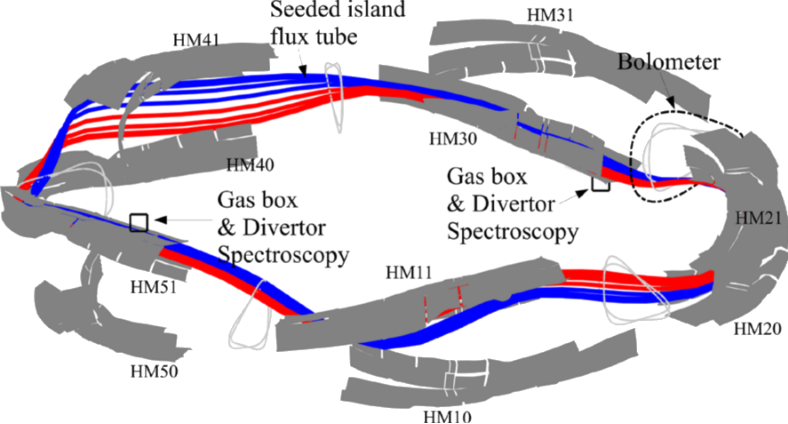
\includegraphics[width=\textwidth]{%
                    content/figures/chapter2/divertor_effenberg_reduced.pdf}%
            \end{subfigure}%
            \caption{\textbf{(left)}: Standard magnetic configuration last closed flux surface (transparent, grey) inside ten divertor modules assembly (dark red). Five flux tubes that helically revolve around the core plasma and follow the island chains in front of the divertors included (red, yellow, purple, green, blue)\cite{Reimold2021}. \textbf{(right)}: Ten divertor elements (half-module HM 1-5, up (1) and down (0)) and helium beam gas boxes with positions of bolometry system (108$^{\circ}$ toroidally) and field lines that connect at the seeding points (red, blue)\cite{Effenberg2019_seed}}\label{fig:divertors_fluxtubes}%
        \end{figure}%
%
        Hereafter presented experiments took place after the aforementioned boronisations and were performed, if not mentioned otherwise, in magnetic \textit{standard high mirror} configurations with a \textit{rotational transform} $\iota=5/5$ \cite{Geiger2014,Effenberg2019_seed}. Five individual island bands wrap around and enclose the magnetically confined plasma region in toroidal direction. The magnetic island chains circle helically between upper and lower divertor elements around the torus, which cut through the enclosing field lines and corresponding separatrices in poloidal direction\cite{Mayer2020}. \autoref{fig:divertors_fluxtubes} shows the assembly of the ten divertor elements. On the left, each coloured band represents an island chain that revolves around the confined plasma region and cycles between upper and lower divertors in consecutive half-modules\cite{Reimold2021}. The right shows the five half modules, which each contain an upper and lower divertor, HM10/1 through HM50/1 respectively. Red and blue bands around the torus indicate traced field lines that originate and terminate in target elements, where the thermal helium beam box is located and gas is injected into the scrape-off layer. Both traces have a target-to-target connection length in the order of $\mathcal{O}$(\SIrange{100}{1000}{\meter}) and follow field lines from one (upstream) divertor, in clockwise (red) and counter-clockwise (blue) direction, until they reach another (downstream) target\cite{Effenberg2019_seed}.%
%
        \subsubsection*{Thermal Helium Beam Diagnostic}%
%
            The line ratio spectroscopy of helium is used to measure electron density and temperature in the scrape-off layer and plasma edge. Due to the intrinsic nature of the fully optimized stellarator W7-X, very low temperatures and densities in divertor regions, especially under conditions of plasma detachment, are expected. Therefore, the spectroscopy is extended by seeding of extrinsic impurities through thermal gas injection valves. These low-Z impurities include helium, neon, argon, methane (CH$_{4}$) and mixtures thereof. Due to their lower excitation energies, the yield of line radiation at low temperatures is much better\cite{Barbui2016}. Electron temperature $T\ix{e}$ and density $n\ix{e}$ can be derived from the ratio of line radiation intensities of atomic helium, which are based off of calculations for emission rate coefficients from a collisional-radiative model.\cite{Denkelmann1999,Krychowiak2011}. The thermal helium beam diagnostic consists of two \textit{in vacuo} boxes at different toroidal locations in one upper lower divertor element. Each is equipped with five, millisecond fast piezo valves that allow for independent gas injection of He, Ar, Ne, N$_{2}$, H$_{2}$ or CH$_{4}$. The nozzles on the gas lines are mounted behind the target elements and directly seed into the same island chain of the $\iota=5/5$ magnetic standard configuration. Line pressures range from a few \SI{}{\milli\bar} to a maximum of \SI{60}{\bar}, where the latter is used for seeding experiments, at around \SI{1.5}{\kilo\meter\per\second} exit velocity and an opening angle of 40$^{\circ}$.\cite{Krychowiak2011,Barbui2016}\\%
%
        \begin{figure}[t]%
            \centering%
            \begin{subfigure}{0.42\textwidth}%
                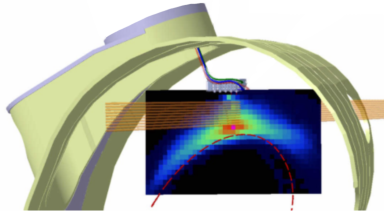
\includegraphics[width=1.0\textwidth]{%
                    content/figures/chapter2/hebeam_box_cut.pdf}%
                \caption{Thermal helium beam and spectroscopy%
                }\label{fig:hebeam}%
            \end{subfigure}%
            \hfill%
            \begin{subfigure}{0.55\textwidth}%
                \includegraphics[width=1.0\textwidth]{%
                    content/figures/chapter2/%
                    divertor_elements_boxes_fs_bw_add_extra.pdf}%
                \caption{Toroidal diagnostic locations}\label{fig:positions}%
            \end{subfigure}%
            \caption{\textbf{(a)}: Gas injection box at the upper plasma edge with all 5 capillary nozzles as used for divertor operation. Included are spectroscopy lines of sight (orange) perpendicular to the beam and the last closed flux surface (red). Superimposed is the result of one EMC3-EIRENE for He line emission\cite{Barbui2016}. \textbf{(b)}: Relative toroidal position of all involved diagnostics. One filterscope system is located in the same divertor as one of the gas valve boxes, while interferometer and electron cyclotron measurements are done in different locations.}\label{fig:hebeam_pos}%
        \end{figure}%
%
        \newline%
        However, the measurement of electron density and temperature in the divertor region by line ratio spectroscopy is of no concern for the plasma feedback control. The fast acting gas valves of the thermal helium beam diagnostic will be used as an actuator for the injection of extrinsic impurities. Other diagnostics provide experimental information that will be used for the feedback system, which ultimately controls the gas boxes. One of those diagnostics is the dispersion interferometry that provides line integrated core plasma densities in real-time.
%
        \subsubsection*{Dispersion Interferometry}%
%
            Interferometry is a fundamental measurement technique to assess the line integrated plasma density. Due to its simple methodology, it is a prime candidate for reliable real-time feedback\cite{Mlynek2010,Boboc2012}. An easily tunable laser is split via a frequency doubling crystal. Both beams pass the plasma co-linearly. Because of their differing group velocities, i.e.dispersion of the plasma with its density dependent refractive index, both beams experience different phase shifts based on the plasma density along their path. After a second pass through the crystal, their interference image can be used to calculate the line integrated density. The disadvantages of this, generally very robust measurement method, are phase shifts that are introduced via perturbations perpendicular to the beam direction and potentially unfavourable SNR due to both reference and measurement beam passing the plasma\cite{Knauer2016}. For the single channel integral electron density dispersion interferometer (IEDDI), a real-time evaluation system based on FPGAs has been implemented. This assembly is capable of providing density measurements with a \SI{23}{\micro\second} latency, which is dominated by the laser diodes modulation. This has a maximum data rate of \SI{50}{\kilo\hertz}. However, the density feedback frequency is mandated by the internal W7-X system at \SI{1}{\kilo\hertz}. The latter is used for feedback by the central stellarator control system and plasma fuelling\cite{Spring2017}. The density data is forwarded with an error of \SI{2e18}{\per\square\meter} and signal drift of \SI{6.7e15}{\per\cubic\meter\per\second} from the last performed laser and phase calibration\cite{Brunner2018}.\\%

        \,\newline%
        Besides the dispersion interferometry, there are two other possible candidates for thermal helium beam feedback. One of them is the spectroscopic imaging system, which measures impurity heat and particle fluxes from the plasma onto the divertor target. It can provide spatial-temporally resolved impurity line radiation, e.g. of carbon species like C$^{2+}$, for feedback purposes.%
%
        \subsubsection*{Filterscope and IR-visible Camera System}%
%
            Two divertor targets have been under special investigation by the spectroscopic imaging system at W7-X in past experimental campaigns\cite{Stephey2016}. In one toroidal position, a combination of high resolution visible-infrared cameras and filterscope systems were able to provide the totally calibrated, spatially and temporally resolved line radiation intensity of H$_{\alpha}$, H$_{\beta}$, He-I, He-II, C-II and C-III from and in front of the target. The filterscopes at W7-X are based on the design from the \textit{Oak Ridge National Laboratory}\footnote[1]{ORNL; Oak Ridge National Laboratory, Oak Ridge, Tennessee, United States of America; 37831-8072}. Lenses located outside the vacuum vessel focus light from the plasma and divertor onto a linear array of optical fibres. At focus lengths of \SI{25}{mm} and \SI{50}{\milli\meter}, the spatial resolution at the target becomes \SI{3.6}{\centi\meter} and \SI{7.1}{\centi\meter}, respectively. Those fibres are connected outside the machine to individual optical bandpass filters, which are attached to photomultiplier tubes (PMT), whose full-width at half maximum is \SIrange{1}{3}{\nano\meter} for the above emission lines. Data acquisition with a temporal resolution of \SI{100}{\kilo\hertz} is taken care of by a LabVIEW\textsuperscript{\textregistered} control program. The filterscopes provided measurements of H$_{\alpha}$, H$_{\beta}$, He-I, He-II, C-II lines and visible bremsstrahlung\cite{Stephey2016}. For feedback purposes, the filterscope system has to provide the accurate photon flux as the brightness of the scrape-off layer changes, which challenges the PMT voltage control. In certain scenarios, relative errors as high as 20\% after gain normalization can occur. For fast plasma transitions with large increments in emission brightness, occasional clipping of the filterscope signal is unavoidable\cite{Colchin2003,Brooks2008}.\\%
            The infrared-visable imaging system is based on the design from the \textit{Los Alamos National Laboratory}\footnote[1]{LANL; Los Alamos National Laboratory, Los Alamos, New Mexico, United States of America}. It is located outside the vacuum vessel as well, while looking at the divertor plasma from \SI{1.5}{\meter} away through a \SI{21.5}{\centi\meter} diameter, \SI{6}{\milli\meter} thick sapphire vacuum window. The infrared camera is acquiring between wavelengths of \SIrange{3}{5}{\micro\meter} at a \SI{125}{\hertz} acquisition rate of 1344$\,\times\,$784 pixel resolution images. The calibration of the camera was performed with a \SI{50}{\milli\meter} or \SI{200}{\milli\meter} lens for temperatures of up to \SI{1200}{\celsius}. In contrast, the visible system is acquiring 1024 pixel square images at \SI{100}{\hertz} with only a \SI{50}{\milli\meter} lens. Both cameras achieve a \SI{1}{\milli\meter} spatial divertor resolution\cite{Wurden2016}.\\%
%
        \,\newline%
        After characterising the dispersion interferometry and filterscopes as candidates to control the , one additional constraint to the performance of the thermal helium beam valve box was made. The central line integrated electron temperature needs to be above \SI{2}{\kilo\electronvolt} in order to avoid poor ECRH coupling and therefore radiation collapses. The electron cyclotron diagnostic (ECE) is measuring line integrated $T\ix{e}$ along a line of sight through the plasma core and along the separatrix, closer to the edge\cite{Krychowiak2021,Hirsch2019,Marushchenko2006}.\\%
        Finally, the real-time radiation feedback system, which provides information about the total radiative power loss of the plasma to the thermal helium beam, will be introduced.%
%
    \section{Real-Time Radiation Feedback System}\label{sec:realtime_radiation}%
%
        The goal of the real-time feedback system is to provide an estimate of $P\ix{rad}$, as derived in \cref{eq:prad_total}, for each sample during data acquisition, with as small as possible latency to the underlying measurement. This means a calibrated, error and offset corrected, filtered absorber voltage $\Delta\widetilde{U}\ix{M}$ needs to calculated within one signal integration cycle. Assuming current results from the \textit{in-situ} calibration routine are available, one is able to find the power onto the absorber for every point in time $P_{M}$, as described by \cref{eq:bolometer_adv}. In order to calculate a total radiation power loss in real-time from $P_{M}$, information about the line of sight geometry have to be provided via $K_{M}$ and $V_{M}$. For an extrapolation of $P\ix{rad}$ similar to \cref{eq:prad_total}, the calculation of geometric coefficients is too computationally expensive and can not be performed during the data acquisition. Therefore, $K_{M}$ and $V_{M}$ have to be provided beforehand, limiting their specificity towards the experiment scenario, e.g. in regard to the magnetic configuration. Finally, due to computational limits, $P\ix{rad}$ of the full HBC or VBC arrays can not be calculated within one sample period. Simplifications to \cref{eq:prad_total} have to be made to achieve a real-time proxy of the radiation power loss. Assume there exists a collection of lines of sight $S$ that measure the radiation power loss from the plasma, so that%
%
        \begin{align}%
            V_{S}=&\sum_{M}^{S}V_{M}\,\,,\nonumber\\%
            \Aboxed{%
                P\ix{pred}^{\left(1\right)}\coloneqq&P_{\text{rad}, S}=\frac{V\ix{P,tor}}{V_{S}}\sum_{M}^{S}\frac{P_{M}V_{M}}{K_{M}}\,\,,\qquad S\subset\left(S\ix{HBC},S\ix{VBC}\right)%
            }\label{eq:prediction}%
        \end{align}%
%
        the predictive value $P\ix{pred}^{\left(1\right)}\approx P\ix{rad}$ the full set of information. An equivalent requirement is the adequate description of the local emissivity distribution by the set of lines of sight $S$, though this abstract concept is difficult to quantitatively assess from the standpoint of the bolometer diagnostic alone. However, an attempt for a rigorous and thorough investigation of the accuracy and reliability of $P_{\text{rad}, S}$ is made in the later \cref{sec:evalmetrics}. The subset $S$ of the total selection of lines of sight, which are available through the HBC and VBC arrays, needs to be much smaller than the main cameras in order to be a candidate for radiation feedback. A decreased amount of channels for calculation means less computational load and therefore promises feasibility for real-time application. A key distinction between $P\ix{rad}$ and $P\ix{pred}^{\left(1\right)}$ is that the prediction has to be limited between \SIrange{0}{10}{\mega\watt}.%
%
        \begin{align}%
            P\ix{pred}^{\left(n\right)}&\in\left(0, 10\right)\,\text{MW}\,\,,\nonumber\\
            U_{\text{AO},n}\left[\,\text{V}\,\right]&=P\ix{pred}^{\left(n\right)}\left[\,\text{MW}\,\right]\,\,,\qquad n=\left\{1,2\right\}\nonumber%
        \end{align}%
%
        On one hand, this is due to the analogue output limitation of the hardware to a range of \SIrange{0}{10}{\volt}. On the other, radiation power loss estimations $>\,$\SI{10}{\mega\watt} for a total possible heating power of \SI{10}{\mega\watt} do not make sense for the aspired feedback system and its requirements. In \cref{eq:prediction}, the analogue output voltages that are used to provide feedback to the gas valve control are noted as $U\ix{AO, n}$, with $n=\{1,2\}$.\\%
        The performance of the real-time radiation system, especially with respect to latency, is crucial to the achievement of stable plasma detachment through hydrogen gas injection in the scrape-off layer. A calculation like in $P\ix{pred}^{\left(1\right)}$ takes a certain, non-negligible amount of computation cycles and time, which inevitably increases the latency of the feedback response, relative to the acquisition of the underlying samples. One way around this issue is to make further simplifications to the approach of \cref{eq:prad_total} or \cref{eq:prediction}. In steady state scenarios, with slow perturbations and small gradients in the radiation power distribution, let us assume:%
%
        \begin{align}%
            &P\ix{M}=F_{M}\left(\frac{\diff\left(\Delta\widetilde{U}_{M}\right)}{\diff t}+f_{M}\Delta\widetilde{U}_{M}\right)\approx F_{M}f_{M}\Delta\widetilde{U}_{M}\,\,,\nonumber\\%
            \Aboxed{%
                &P\ix{pred}^{\left(2\right)}\coloneqq\frac{V\ix{P, tor}}{V_{M}}\cdot\frac{P_{M}V_{M}}{K_{M}}\overset{!}{=}a_{M}\Delta\widetilde{U}_{M}\,\,,\qquad M\in\left(S\ix{HBC}, S\ix{VBC}\right)%
            }\label{eq:prediction2}%
        \end{align}%
%
        \autoref{eq:prediction2} yields a different approach to the radiation power loss proxy. Assumptions for $P\ix{pred}^{\left(2\right)}$ require $\diff\Delta\widetilde{U}_{M}/\diff t\ll f_{M}\Delta\widetilde{U}_{M}$ and therefore temporal changes in the radiation distribution to be negligible. This saves additional computational steps by eliminating the derivative. Furthermore, removing the sum in \cref{eq:prediction} assumes the radiation to be located mainly in or around one radial position, i.e.one point in the chord brightness profile, which is symmetrically distributed in poloidal and toroidal direction. The channel constant $a_{M}$ can be calculated in advance to the measurement. For example: with $R_{M}=\text{\SI{1}{\kilo\ohm}}$, $\tau_{M}=\text{\SI{110}{\milli\second}}$ and $\kappa_{M}=\text{\SI{0.8}{\milli\watt/\kilo\ohm}}$, which gives $F_{M}=0.343$ and $f_{M}=0.993$, $K_{M}=\text{\SI{1.1e-10}{\cubic\meter}}$ and a total radiating plasma volume $V\ix{P, tor}=\text{\SI{45}{\cubic\meter}}$, the channel constant to upscale the absorber voltage $\Delta\widetilde{U}_{M}$ to feedback proxy becomes $a_{M}=\text{\SI{141.18}{\mega\watt\per\milli\volt}}$. At an absorber signal of $\Delta\widetilde{U}_{M}=\text{\SI{0.1}{\milli\volt}}$, \cref{eq:prediction} will estimate and extrapolate a total plasma radiation of $P\ix{pred}^{\left(2\right)}=\text{\SI{1.41}{\mega\watt}}$.\\%
        \autoref{eq:prediction} will be the reference for a radiation power loss proxy that can be implemented for the scrap-off layer seeding system. Nevertheless, both of the previously introduced concepts have been used during the last experimental campaign to provide radiation power loss predictions. Details of how the implemented diagnostic hardware and a tailored algorithm calculated the radiation power proxy will be described below.\\%
        To start, the setup that was used to provide radiation loss information to the thermal helium beam box will be introduced. The center component of the bolometer feedback system is the PCI Express add-in card and multipurpose input/output device NI\textsuperscript{\textregistered} 6321. For the purposes of this experiment, only the analogue output capabilities of this device are of interest. The cards specifications have been rated for constant environmental conditions, i.e. temperature and humidity, which are provided by the air-conditioned cabinet in the torus hall, where the bolometer system PC this device has been installed on is located. The NI\textsuperscript{\textregistered} 6321 incorporates two analogue output channels that are both able to provide a DC coupled voltage signal in the range of $\pm$\SI{10}{\volt}, with 16$\,$bit or \SI{0.3}{\milli\volt} resolution. If both channels are being used, the maximum update rate becomes \SI{840}{\kilo\sample\per\second}, which is equal to a \SI{1.2}{\micro\second} sample time with an accuracy of \SI{10}{\nano\second}. The output has a buffer array of 8191$\,$samples, where the first sample in is replaced by sample number 8191+1 and so on (FIFO\footnote[1]{FIFO: First In – First Out}, see \cref{fig:fifo}). The absolute error $\Delta U\ix{AO}$ for output voltage $U\ix{AO}$ of the device is given by:%
%
        \begin{align}%
            \begin{split}\label{eq:output_accuracy}%
                \Delta U\ix{AO}=\,\,&U\ix{AO}\Delta G+R\Delta U\ix{off}\\%
                &\Delta G=\sigma\ix{G}+s\ix{G}\Delta T\ix{in}+s\ix{r}\Delta T\ix{ex}\\%
                &\Delta U\ix{off}=\sigma\ix{off}+s\ix{off}\Delta T\ix{in}+\Delta\text{INL}\,\,,\\%
            \end{split}%
        \end{align}%
%
        where $\Delta T\ix{in}$ and $\Delta T\ix{ex}$ are the temperature difference to the last internal and external calibrations, and $R$ the set output range of the card. The noted properties and their value can be found in \cref{tab:output_accuracy}. For a temperature change relative to the calibrations of \SI{1}{\celsius} and \SI{5}{\celsius} respectively, an output range of \SI{20}{\volt} ($\pm\,$\SI{10}{\volt}) and voltage of $U\ix{AO}=\,$\SI{1}{\volt} the analogue error becomes $\Delta U\ix{AO}\approx\,$\SI{3}{\milli\volt}. The characterisation of the hardware will later be put into context when addressing the performance and limits.\\%
%
        \begin{table}[t]%
            \centering%
            \begin{tabular}{||c|c|c|c||}%
                \hline\rule{0pt}{.75\normalbaselineskip}%
                property & $\sigma\ix{G}$ & $s\ix{G}$ & $s\ix{r}$ \\[.5ex]\hline\hline%
                value & $8\times\tenpo{-5}$ & \SI{1.13e-5}{\per\celsius} & \SI{5e-6}{\per\celsius} \\[.5ex]\hline%
            \end{tabular}%
            \,\\[.5ex]%
            \begin{tabular}{||c|c|c|c||}%
                \hline\rule{0pt}{.75\normalbaselineskip}%
                property & $\sigma\ix{off}$ & $s\ix{off}$ & $\Delta\text{INL}$ \\[.5ex]\hline\hline%
                value & $5.3\times\tenpo{-5}$ & \SI{4.8e-6}{\per\celsius} & $1.28\times\tenpo{-4}$ \\[.5ex]\hline%
            \end{tabular}%
            \vspace*{0.5cm}%
            \caption{Output and temperature characteristics of NI\textsuperscript{\textregistered} 6321.}\label{tab:output_accuracy}%
        \end{table}%
%
        The NI\textsuperscript{\textregistered} 6321 is only tasked with providing signals for the gas valve control. Therefore, the procedure of acquisition and the algorithm that are responsible for real-time feedback need to be presented next. In \cref{subsec:construction}, the bolometry system has been described. The following introduction builds on the specifications of the previously implemented system.
%
        \subsubsection*{Measurement Algorithm}%
%
            Assume an incoming signal that functions as an event trigger, as is standard for the central W7-X control system, which marks the point in time $T0=T1-\,$\SI{60}{\second}, with $T1$ being the moment the experiment starts - commonly the startup of ECRH microwaves\cite{Spring2017}. A bare bone, top level LabVIEW program, designated to receiving and interpreting any incoming trigger signals as fast as possible, is forwarding a start command to the core bolometer control. The trigger routine is executed before an experiment session and is running with the lowest possible latency, which is $\ll\,$\SI{1}{\milli\second}. The initialization of the main bolometer LabVIEW routine is following the start signal from the trigger program. The user interface input parameters, which have been set before runtime, are stored in memory for later requests during execution. This includes links to local files containing the line of sight geometry. Thereby provided $K\ix{M}$ and $V\ix{M}$ are, for reasons stated above, derived from magnetic standard configuration calculations.\\%
            A preventative reset and clearing of the bit registers and FPGA states of the NI\textsuperscript{\textregistered} AD 7730 is carried out in the beginning of the execution. For each of the following internal routines, the bit programmable registers, which are responsible for the mode, voltage range and frequency of acquisition, are set to appropriate values. For the initial floating potential measurement, which has been mentioned in \cref{subsec:bolometerequations}, the device is put into full range mode, i.e. $\pm\,$\SI{80}{\milli\volt} and sample frequency of \SI{0.4}{\milli\second}. The subsequent measurement of \SI{10}{\second} yields the offset voltage and measurement noise per channel. Next, the registers are reset again and then put into calibration mode, which enables the NI\textsuperscript{\textregistered} AD 7730 to measure the current through individual parts of the Wheatstone bridge. As lined out in \cref{sec:w7xbolometer}, a calibration routine incorporating two subsequent heating stages with \SI{1.2}{\volt} and \SI{2.5}{\volt} for \SI{1.6}{\second} each is then executed. Resulting currents are measured with a sampling time of \SI{0.4}{\second}. This, in total \SI{4}{\second} long procedure is repeated for both of the reference and measurement parts of the Wheatstone bridge. In succession to the four individual calibration routines, the respective properties $\kappa$, $\tau$ and $R$ for reference and measurement absorbers are calculated using \cref{eq:resistance} and following (see \cref{subsec:bolometerequations}). Thereafter, filter and mode register are programmed to continuously acquire $N$ data points at the given sample time of \SIrange{0.8}{6.4}{\milli\second} for the measurement of experiment data. At this point, the program indicates a total runtime of \SIrange{25}{30}{\second}, depending on small changes in the PCs execution prioritisation. The remaining part of the $T0\,+\,$\SI{60}{\second}$\,\rightarrow T1$ section is downtime.\\%
            Simultaneously, the NI\textsuperscript{\textregistered} 6321 is programmed for two-channel analogue output. A global variable for each channel, i.e. memory address for writing and reading is provided beforehand. The most current radiation values are calculated using $P\ix{pred}^{\left(n\right)}$ from \cref{eq:prediction} and \cref{eq:prediction2} individually, inside the acquisition routine, which will be presented further down below. The addresses are read from inside a loop structure separate from the acquisition, which runs as fast as allowed by the output performance of the card.\\%
%
            % \begin{figure}[t]%
            %     \centering%
            %     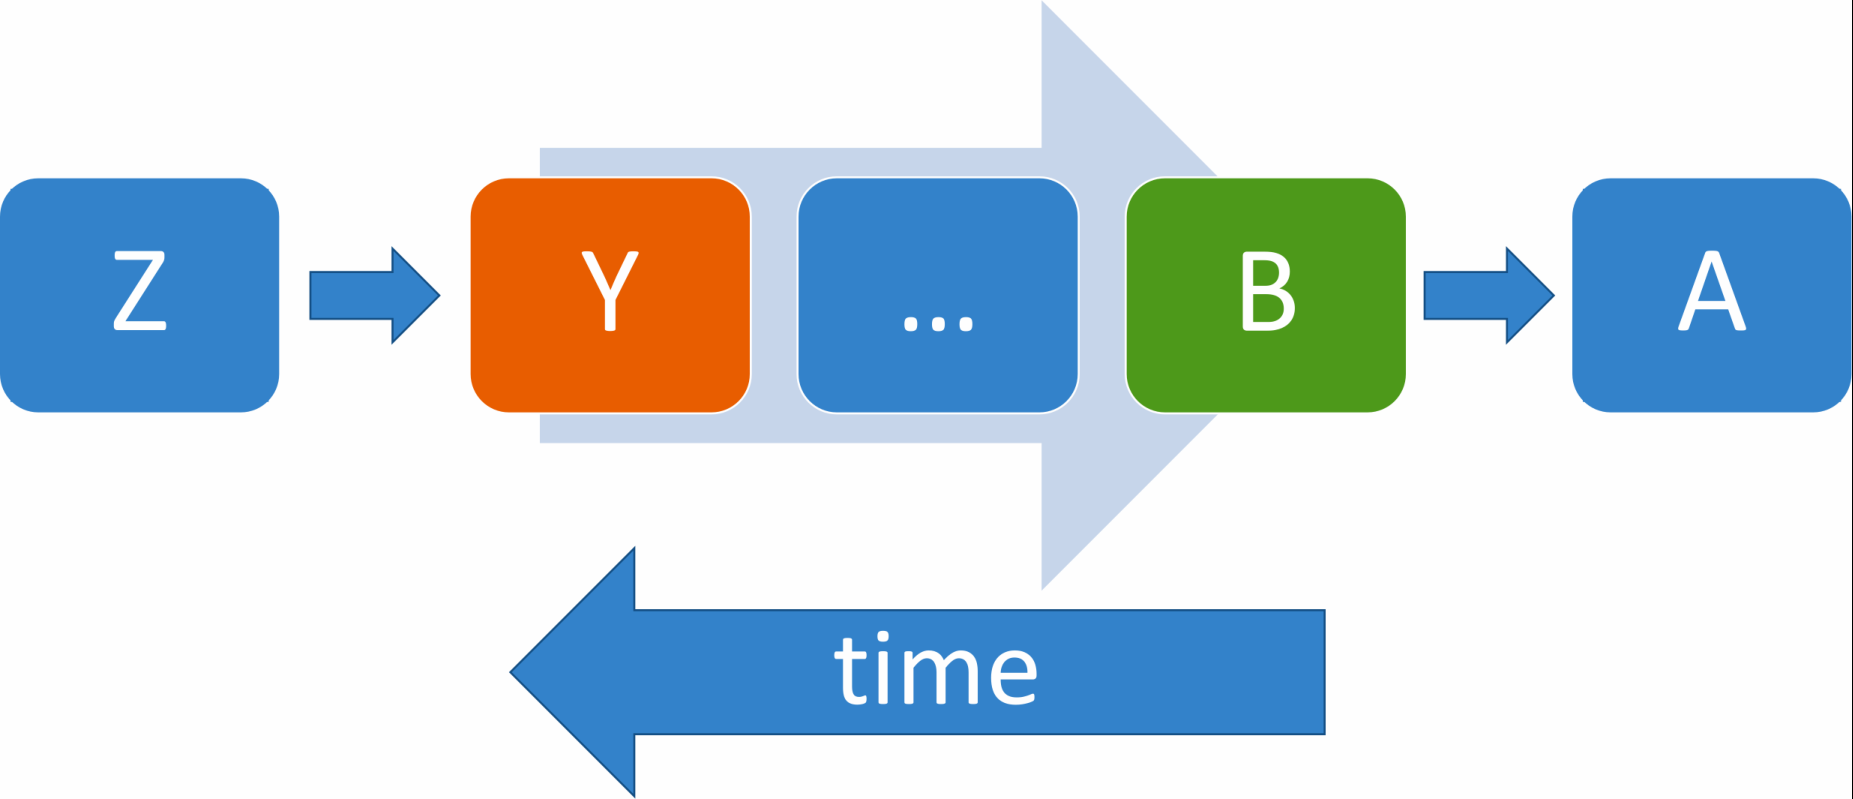
\includegraphics[width=0.5\textwidth]{%
            %         content/figures/chapter2/fifo.pdf}%
            %     \caption{Schematic of a FIFO array. Time progresses from right to left, i.e. sample A is acquired before B, \dots, Y and Z. Currently stored samples are B, \dots, Y. When sample Z is acquired, sample A is removed from the FIFO array, the oldest data point at this moment.}\label{fig:fifo}
            % \end{figure}%
%
            A certain amount of time, e.g. \SI{5}{\second} before $T1$, the system starts acquiring samples. The main LabVIEW program initialises a sub-routine that only takes care of data acquisition. Required storage arrays and memory addresses are either referenced or created at first runtime. In scenarios where no feedback is required, only the raw data is returned from the sub-routine, with no additional tasks performed during sample cycles. Also, the initialisation of the NI\textsuperscript{\textregistered} 6321 is omitted. For feedback purposes, multiple additional arrays have to be prepared. The raw samples $\Delta U_{M}$ of channels that are in the selection $S$ are stored in an array with the number of rows $\vert S\vert$, the cardinality of the subset. In order to reduce the impact of signal noise on the prediction value, smoothing like in \cref{eq:averaging} has to be applied. In real-time application, performing a full width Savitzky-Golay filter the width of $L$ samples for each channel is not possible. A computationally affordable approach to a boxcar filter is the FIFO array. Consecutive samples are stored in a container of length $L+2$. Assume an iterator $i$ that counts the progression of data points in time. For $i\le L$ samples are placed in the container at index $i$. Once the iterator reaches $i>L$, the stored samples are replaced by new ones at their location $j\equiv i\pmod{L}$, hence \textit{first in - first out}. For $i=M$, the mean over all elements is stored in column $L+1$. In the next iteration, entry $L+1$ is moved to column $L+2$ and the new mean is calculated in $L+1$. This is repeated in all following cycles. Hence, data of the real-time feedback algorithm is stored in a structure the size $\vert S\vert\times\left(L+2\right)$.\\%
            After the required memory space and addresses have been reserved, the data acquisition is started. The enclosing loop over $N$ repetitions is timed by the length of a sample, e.g. \SI{1.6}{\milli\second}. An acquired data point $\Delta U_{M}^{\left(i\right)}$ for sample number $i$ is subtracted by the previously in-situ measured offset $V_{\text{off}, M}$ and stored in the FIFO array at its corresponding location. After $M$ iterations and onwards, for every sample $i$ and channel $M$, the boxcar filtered $\Delta\widetilde{U}_{M}^{\left(i\right)}$ is calculated. The temporal derivative is calculated from columns $L+1$ and $L+2$ using the discrete \textit{forward Euler\footnote[1]{Leonhard Euler *~Apr. 15. 1707 \textdagger~Sept. 18 1783} method}:%
%
            \begin{align}%
                \frac{\diff\left(\Delta\widetilde{U}_{M}^{\left(i\right)}\right)}{\diff t}\approx\frac{\Delta\widetilde{U}_{M}^{\left(i\right)}-\Delta\widetilde{U}_{M}^{\left(i-1\right)}}{\Delta t}\,\,.\nonumber%
            \end{align}%
%
            Note however that this explicitly not apply to $P\ix{pred}^{\left(2\right)}$, where the derivative is omitted.\\%
            By referencing the current calibration results, one finds $P_{M}^{\left(i\right)}$ from the last and second to last column of the FIFO array using \cref{eq:bolometer_adv}. With $K_{M}$ and $V_{M}$ provided through input files, the final step is done in \cref{eq:prad_total}, which yields $P\ix{rad}=P\ix{pred}^{\left(1\right)}$. Similarly, $P\ix{pred}^{\left(2\right)}$ is derived from a separate FIFO array which only stores samples of one channel. The scaling factor $a_{M}$ is calculated beforehand.\\%
            For each iteration $i>L$, both $P\ix{pred}^{\left(n\right)}$ are written to their respective memory addresses, which are read from in the top-level routine, where the analogue output is carried out as fast as possible. Also, both values are written to individual arrays that are returned to the main program after the measurement loop has been completed. After $N$ samples, $P_{M}$, $\Delta U_{M}$ and both $P\ix{pred}^{\left(n\right)}$ are forwarded to the primary LabVIEW application. The measurement procedure has been successfully completed at this point. Output loop and device status are reset and returned to default for the next experiment. At last, the data will be stored locally and uploaded to the central W7-X archive, including the calibration currents, results and feedback proxies. Measurement, as well as feedback routine and algorithm are shown in a schematic outline in \cref{apx:algorithm} by \autoref{alg:algorithm}.\\%
            The performance of the \textit{real-time radiation feedback system} has been tested and benchmarked before its application during the experimental campaign. An uncalibrated diode laser with \SI{7}{\milli\watt} continuous power output was aimed at a single detector absorber, like it was described in \cref{subsec:construction}, outside the plasma vessel and inside the measurement cabinet of the bolometer diagnostic. A frequency generator with cycle frequencies of \SI{1}{\hertz}-\SI{1}{\kilo\hertz} and output voltages $<\SI{10}{\volt}$ has been powering the laser diode. The detector was connected to a vacant port in the acquisition electronics. In order to find the intrinsic, lowest possible latency of the system, the length of the \textit{FIFO} buffer was set to the minimum $M=1$. A measurement program was carried out while the laser was adjusted to its maximum \SI{7}{\milli\watt} intensity at a square wave cycle frequency of \SI{1}{\hertz}. The output of the frequency generator was split between the diode and one input of an oscilloscope. The prediction $P\ix{pred}^{\left(1\right)}$ for the analogue output was calculated using \cref{eq:prediction} and was also monitored by the oscilloscope with a separate input. The result of the benchmark can be seen in \cref{fig:oscilloscope}. A minimum intrinsic latency of the system of \SI{13.6}{\milli\second} was achieved. Prediction and analogue output using $P\ix{pred}^{\left(2\right)}$ resulted in the same values. Further temporal delays are subject to the smoothing of the FIFO array over $M$ samples of length $\Delta t$:%
%
            \begin{align*}%
                \Delta T\approx\frac{M\cdot\Delta t}{2}\,\,.%
            \end{align*}%
%
            In context of the other feedback candidates and actuator system, this latency is the largest among the individual diagnostics. This will become important when discussing initial results of the bolometer feedback and comparing its achievements to the results other control values.%
%
            \begin{figure}[t]%
                \centering%
                \includegraphics[width=0.5\textwidth]{%
                    content/figures/chapter2/oscilloscope_fix.pdf}%
                \caption{Real-time feedback system benchmark result for \SI{7}{\milli\watt} at \SI{1}{\hertz} \textbf{laser} diode power and frequency. The \textbf{detector} response was created using the algorithm for $P\ix{pred}^{\left(1\right)}$ with $M=1$ the FIFO array length. A total, minimum latency of \SI{13.6}{\milli\second} was achieved during the test.}\label{fig:oscilloscope}%
            \end{figure}%
%
            \subsubsection*{PID Controller}%
%
                % \begin{figure}%
                %     \centering%
                %     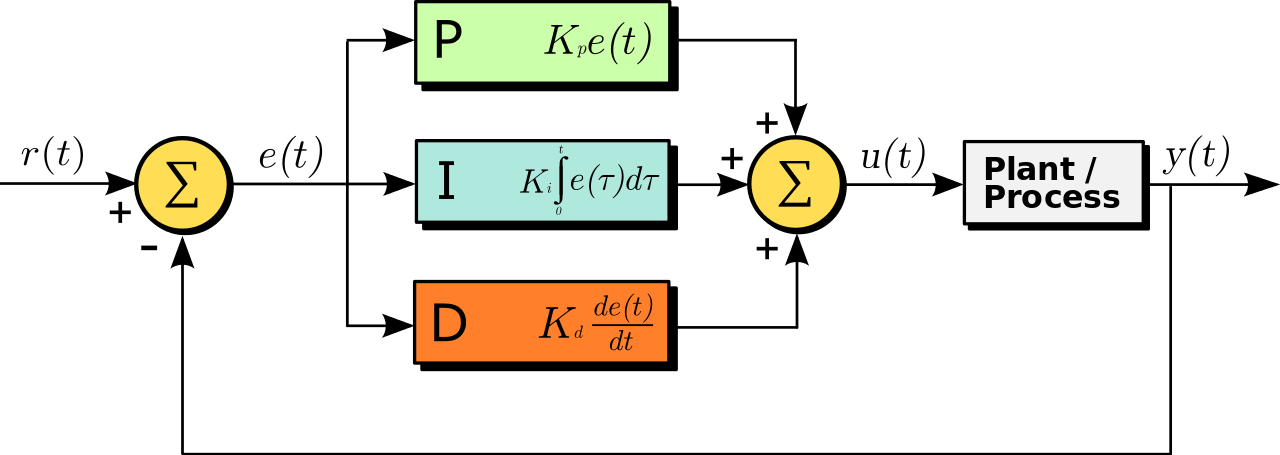
\includegraphics[width=0.7\textwidth]{%
                %         content/figures/chapter2/PID_en.png}%
                %     \caption{A block diagram of a PID controller in a feedback loop. Desired process value or setpoint SP $r\left(t\right)$ and measured process value PV $y\left(t\right)$. The control function $u\left(t\right)$ is used for feedback\cite{WikiPID}.}\label{fig:pid}
                % \end{figure}%
%
                Both of the analogue output channels of the NI\textsuperscript{\textregistered} 6321 that provide $P\ix{pred}^{\left(n\right)}$ are connected via individual, BNC\footnote[1]{BNC: Bayonet Neill Concelman, Bayonet Nut Connector or British Naval Connector} terminated, double shielded cables outside the vacuum vessel to an \textit{Arduino}\footnote[2]{open-source electronics platform, based on easy-to-use hardware and software for I/O} based \textit{PID}\footnote[3]{PID: proportional–integral–derivative controller} that controls the gas valves. In fact, the analogue values of all input diagnostic signals to that device were digitised and passed to the controller over a direct network fibre-optic cable connection. Such a controller is widely used in control systems that incorporate feedback mechanisms. The PID algorithm continuously modulates a control function, based on an error value $e\left(t\right)$ between a setpoint SP$\,\equiv r\left(t\right)$ and process variable PV$\,\equiv y\left(t\right)$. A correction to the feedback control is applied involving a proportional (P), integral (I) and derivative (D) term of $e\left(t\right)$. A setpoint $r\left(t\right)$ is defined as the desired state of the machine or system. The current state of the system is measured in $y\left(t\right)$. Error $e\left(t\right)$ is given by the difference of SP and PV. Individually optimized constants $K\ix{p}$, $K\ix{i}$ and $K\ix{d}$ scale the proportional, integral and differential part of the control function $u\left(t\right)$. The impact of the feedback mechanism, which is controlled by $u\left(t\right)$, is measured in $y\left(t\right)$ and is used for subsequent adjustments to the control. The control function is given by:%
%
                \begin{align}%
                    \begin{split}%
                        e\left(t\right)&=r\left(t\right)-y\left(t\right)\\%
                        u\left(t\right)&=K\ix{p}e\left(t\right)+K\ix{i}\int_{t_{0}}^{t}\,e\left(t^{\prime}\right)\diff t^{\prime}+K\ix{d}\frac{\diff\,e\left(t\right)}{\diff t}\,\,.%
                    \end{split}\label{eq:pid}%
                \end{align}%
%
                \begin{figure}[t]%
                    \centering%
                    \includegraphics[width=\textwidth]{%
                        content/figures/chapter2/pid_example.pdf}%
                    \caption{Example of how the control function $u\left(t\right)$ changes for the same setpoint SP (grey dashed) and system but different proportional, integrals and differential parts.}\label{fig:pid_results}%
                \end{figure}%
%
                \autoref{fig:pid_results} shows how the control function for the same setpoint and response changes with different $K\ix{p}$, $K\ix{i}$ and $K\ix{d}$. The proportional component determines the approach of $u\left(t\right)$ to the setpoint. For larger $K\ix{p}$, the amplitude of the control increases and vice versa, i.e.smaller proportionality leads to a slower adjustment towards the SP. The integral component is responsible for the long-term development of the control. Scaling $K\ix{i}$ up eventually can lead to a faster balancing with the setpoint, but too large values will force the control to underestimate the error more consistently. Smaller differential contributions with $K\ix{d}$ dampen oscillations in the feedback control, but can also neglect and smooth over fast, transitional responses of the system.\\%
                For feedback control with electron density measurements by dispersion interferometry, the factors of proportional and integral part $K\ix{p}$ and $K\ix{i}$ have been individually optimized based on previous measurements and knowledge about delays in the feedback system itself, i.e. valve opening and closing times, data acquisition latency and plasma time scales. A differential component $K\ix{d}=0$ is excluded in those scenarios. During real-time radiation feedback-control, a different, also uniquely optimized set of parameters has been used. In this case, also $K\ix{d}\neq 0$ has been included. For both, there are two sets of PID factors that scale either more aggressively or conservatively.%
%
        \subsection{Performance}\label{sec:drawbacks}%
%
            \begin{figure}[t]%
                \centering%
                \begin{subfigure}{0.48\textwidth}%
                    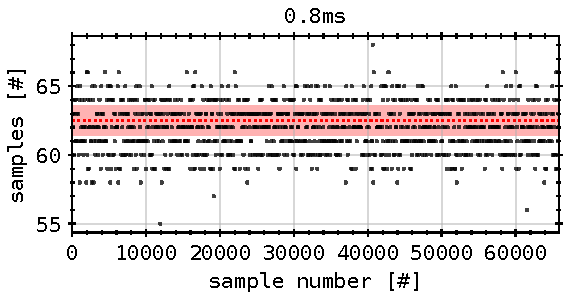
\includegraphics[width=\textwidth]{%
                        content/figures/chapter2/lib_woRTF_branch_nS_0_8ms.pdf}%
                    \caption{samples per half period}
                \end{subfigure}%
                \hspace*{0.25cm}%
                \begin{subfigure}{0.48\textwidth}%
                    \includegraphics[width=\textwidth]{%
                        content/figures/chapter2/lib_woRTF_branch_sT_0_8ms.pdf}%
                    \caption{sample time}
                \end{subfigure}%
                \caption{Laser test results without real-time radiation feedback. The expected number of samples and average sample time are shown in red. \textbf{(left)}: Number of samples per laser half period over sample number \textbf{(right)}: average sample time over laser half period, as derived from the leftover acquisition time.}\label{fig:woRTF_0.8ms}%
            \end{figure}%
%
            % Drawbacks and impact on measurement.
            The previous efforts around the real-time radiation system and underlying algorithm were dedicated to a reliable, low latency performance for detachment control purposes. In order to ensure a consistent sampling of the absorber signal and subsequent radiation power, while also calculating and providing feedback proxies $P\ix{pred}^{\left(n\right)}$, measurements of the acquisition cycle timings was performed. Therefore, the same setup as for the intrinsic latency test of the radiation feedback system was used. An uncalibrated diode laser with \SI{7}{\milli\watt} continuous power output was aimed at a single detector absorber in a laboratory environment, outside the plasma vessel. A frequency generator with \SI{1}{\hertz}-\SI{1}{\kilo\hertz} of $<\SI{10}{\volt}$ output voltages was powering the diode. The exposed absorber was connected to a vacant port in the diagnostic electronics. In order to measure the actual sample times for the individually set $\Delta t$, diagnostic programs were carried out with maximum acquisition length and a square wave signal laser facing the detector. The measurement procedure was performed while the laser was adjusted to its maximum \SI{7}{\milli\watt} intensity with a frequency of \SI{1}{\hertz}. For a set sample time $\Delta t$ and laser half period of \SI{0.5}{\second}, the number of samples that are expected to measure the laser light is given by:%
%
            \begin{align}%
                N=\frac{\SI{0.5}{\second}}{\Delta t}\pm1\,\,.\nonumber%
            \end{align}%
%
            An uncertainty of one sample is assumed, both for errors in distinguishing process of rising and falling slopes in the signal and the smallest possible resolution of the measurement. Rewriting $N$ for $\Delta t$ yields the \textit{actual sample time} for the respective laser half period.\\%
%
            \begin{figure}[t]%
                \centering%
                \begin{subfigure}{0.48\textwidth}%
                    \includegraphics[width=\textwidth]{%
                        content/figures/chapter2/lib_woRTF_branch_sT_1_6ms.pdf}%
                \end{subfigure}%
                \hspace*{0.25cm}%
                \begin{subfigure}{0.48\textwidth}%
                    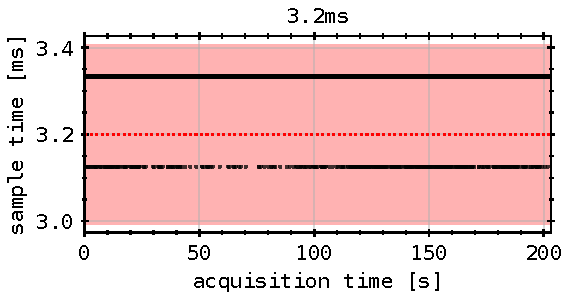
\includegraphics[width=\textwidth]{%
                        content/figures/chapter2/lib_woRTF_branch_sT_3_2ms.pdf}%
                \end{subfigure}%
                \caption{Laser test results without real-time radiation feedback for \SI{1.6}{\milli\second} and \SI{3.2}{\second}. Both show the average sample times per laser half period over acquisition duration. The expected average sample times are shown in red.}\label{fig:woRTF_1.6_3.2ms}%
            \end{figure}%
%
            The results for no real-time radiation feedback, i.e. without the algorithm and calculations related to the proxies, for a set sample time of $\Delta t=\SI{0.8}{\milli\second}$ can be seen in \cref{fig:woRTF_0.8ms}. This is the lowest possible sample time of bolometer data acquisition, regardless of feedback and experiment configuration. The number of data points is limited by the memory of the system. Therefore, for longer periods of acquisition, larger $\Delta t$ have to be selected in order to cover the experiment duration. For $\Delta t=\SI{0.8}{\milli\second}$, the actual sample time is found to be within $\SI{0.05}{\milli\second}$ of the set sample time \SI{0.8}{\milli\second}. A large amount of data points indicate a divergence from the programmed acquisition time $\Delta t$, which is supported by the accompanying number of points per laser half period, which show the same behaviour. This is equal to a 6.25\% error in sample timing, which is significantly larger than the in \cref{subsec:performance} already discussed minimum resolution of ADC programming and physical properties of the absorber design.\\%
            Results for $\Delta t=\SI{1.6}{\milli\second}$ and \SI{3.2}{\milli\second} are shown in \cref{fig:woRTF_1.6_3.2ms}. Similar perturbations of the acquisition timing can be found for \SI{1.6}{\milli\second}, while the spectrum of measured sample times only consists three values. For $\Delta t=\SI{3.2}{\milli\second}$, the results are within the error bar of the measurement and therefore in agreement with the predicted timing. Larger sample times show the same results and therefore support the findings of this benchmark. An erratic error in acquisition sample timing is found for $\Delta t<\SI{1.6}{\milli\second}$, which is presumably caused by the routine of signal integration in LabVIEW$\textsuperscript{\textregistered}$. This specific part of the program is clocked at a fixed frequency for each set sample time $\Delta t$. Interferences can be caused by additional task, which are performed during each sample clock of the actual measurement.\\%
%
            \begin{figure}[t]%
                \centering%
                \begin{subfigure}{0.48\textwidth}%
                    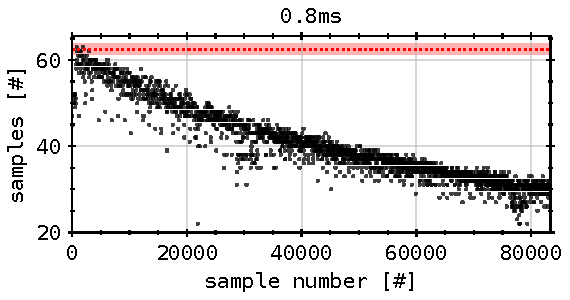
\includegraphics[width=\textwidth]{%
                        content/figures/chapter2/lib_wRTF_branch_nS_0_8ms.pdf}%
                    \caption{samples per half period}
                \end{subfigure}%
                \hspace*{0.25cm}%
                \begin{subfigure}{0.48\textwidth}%
                    \includegraphics[width=\textwidth]{%
                        content/figures/chapter2/lib_wRTF_branch_sT_0_8ms.pdf}%
                    \caption{sample time}
                \end{subfigure}\\%
                \caption{Laser test results with real-time radiation feedback. The expected number of samples and average sample time are shown in red. \textbf{(left)}: Number of samples per laser half period over sample number \textbf{(right)}: Average sample time over laser half period, as derived from the leftover acquisition time.}\label{fig:wRTF_0.8ms}%
            \end{figure}%
%
            In the next step, in order to compare the results without feedback, the same benchmarks are performed for the real-time radiation algorithm. The results for $\Delta t=\SIrangemath{0.8}{1.6}{\milli\second}$ are shown in \cref{fig:wRTF_0.8ms}. From the very first data point and laser period, an increasing sample time is found over the entire measurement duration. The first samples are already substantially longer than the set \SI{0.8}{\milli\second}, while their length only grows with \SI{0.01}{\milli\second\per\second} or \SI{0.01}{\micro\second\per\sample}. This leads to an increase by factor two of the set sample time after \SI{60}{\second} to $\approx\SI{1.6}{\milli\second}$. For $\Delta t=\SIrangemath{1.0}{1.6}{\milli\second}$, similar results can be seen in \cref{fig:wRTF_1.0_1.6ms}. However, an elongation of the sample cycle is found to occur after a certain number of samples have been processed, i.e. $\approx\SI{28000}{\sample}$ for $\Delta t=\SI{1.0}{\milli\second}$. Like before, a linear increase of \SI{0.01}{\milli\second\per\second} in sample length is found from this point onwards. For an even longer sample time of \SI{1.6}{\milli\second}, only single data points deviate from $\Delta t$, while the majority of samples is still within the expected timing window of the program. However, in comparison to the previous results without real-time feedback, $\Delta t=\SI{1.6}{\milli\second}$ exhibits greater uncertainties towards the end of the acquisition. Larger sample times show no perturbations due to the feedback algorithm and its interference with the acquisition cycle.\\%
%
            \begin{figure}[t]%
                \centering%
                \begin{subfigure}{0.48\textwidth}%
                    \includegraphics[width=\textwidth]{%
                        content/figures/chapter2/lib_wRTF_branch_sT_1_0ms.pdf}%
                \end{subfigure}%
                \hspace*{0.25cm}%
                \begin{subfigure}{0.48\textwidth}%
                    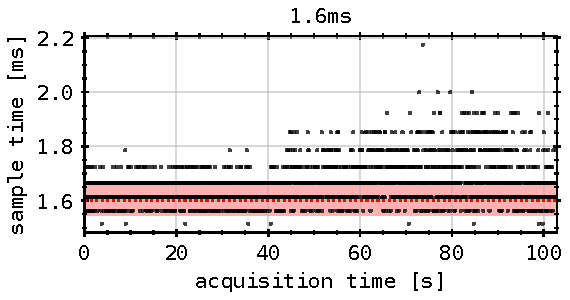
\includegraphics[width=\textwidth]{%
                        content/figures/chapter2/lib_wRTF_branch_sT_1_6ms.pdf}%
                \end{subfigure}\\%
                \caption{Laser test results with real-time radiation feedback for \SI{1.0}{\milli\second} and \SI{1.6}{\milli\second}. Both show the average sample times per laser half period over acquisition duration. The expected average sample time is shown in red.}\label{fig:wRTF_1.0_1.6ms}%
            \end{figure}%
%
            In order to be able to rule out any interference of the PC system on the performance on the acquisition timing, the same benchmarks are repeated with a synthetic load of at least 80\% of its capacity on the central processing unit of the system. If the stress on the computational unit does have any impact on the calculation speed, with which the algorithm is performed, and therefore timing of the diagnostic, a significant increase in deviation from the set sample time $\Delta t$ is expected. The results for $\Delta t=\SI{0.8}{\milli\second}$ are shown in \cref{fig:woRTF_load}. When comparing results to the previously presented measurements without synthetic PC load and real-time feedback, there is no noticeable difference in the number of samples per half period or actual sample time. This is the case for all larger samples times $\Delta t$. The computational stress of the computer is found to have no effect on the performance of the bolometer acquisition.\\%
            The presented results inevitably show that the real-time radiation feedback is not applicable for sample times $\Delta t<\SI{1.6}{\milli\second}$, or at higher acquisition frequencies for experiment times above \SI{30}{\second}. Furthermore, in its current configuration, the bolometer systems acquisition duration is limited by its memory capacity with regard to the selected sample time $\Delta t$. The perturbations in \textit{actual} sample timing can be found for all individual sample time settings $\Delta t$. They show random behaviour and protrude in both directions around the set value with similar amplitudes. Both bolometer acquisition programs, with and without real-time feedback, present erratic divergence of the sample timing. However, the latter shows stretching of integration periods for lower set sample times. No coherent alteration of experimental data timelines due to random perturbations in sample timing is expected. Though, future bolometer measurements could greatly benefit from a similar setup to be permanently installed at the diagnostic.\\%
%
            \begin{figure}[t]%
                \centering%
                \begin{subfigure}{0.48\textwidth}%
                    \includegraphics[width=\textwidth]{%
                        content/figures/chapter2/%
                        lib_woRTF_branch_load_nS_0_8ms.pdf}%
                \end{subfigure}%
                \hspace*{0.25cm}%
                \begin{subfigure}{0.48\textwidth}%
                    \includegraphics[width=\textwidth]{%
                        content/figures/chapter2/%
                        lib_woRTF_branch_load_sT_0_8ms.pdf}%
                \end{subfigure}\\%
                \caption{Laser test results without real-time radiation feedback and additional, synthetic PC load. The expected number of samples and average sample time are shown in red. \textbf{(left)}: Number of samples per laser half period over sample number \textbf{(right)}: Average sample time over laser half period over acquisition time.}\label{fig:woRTF_load}%
            \end{figure}%
%
            The following experimental applications of real-time radiation feedback will incorporate the findings of this benchmark. If not stated otherwise, the set sample time of the bolometer acquisition is \SI{1.6}{\milli\second}.%
%
    \subsection{Experimental Achievements}\label{sec:feedbackachieve}%
%
        % Experimental achievements.%
        After characterising the \textit{real-time radiation feedback} system in the previous section, one can now begin to present and discuss its experimental achievements from the last experimental campaign.%

        \subsubsection*{Initial Results}%
%
            \begin{figure}[t]%
                \centering%
                \captionsetup{width=.45\textwidth}%
                \begin{minipage}[c]{0.45\textwidth}%
                    \caption{Line of sight selection for experiment number XP20180920.29, only containing of HBC channels from the top and center part of the triangular cross-section, i.e. the bolometer measurement plane around $\varphi=108^{\circ}$ toroidally.}\label{fig:20180920.29_channels}%
                \end{minipage}%
                \hfill%
                \begin{minipage}[c]{0.5\textwidth}%
                    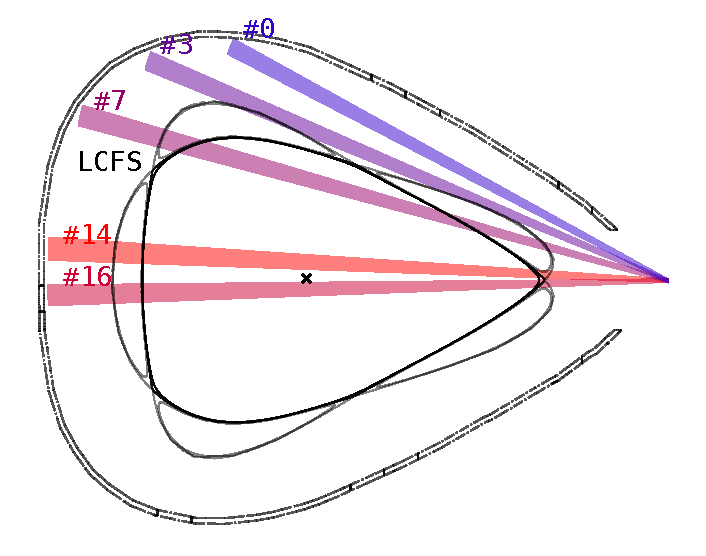
\includegraphics[width=\textwidth]{%
                        content/figures/chapter2/%
                        20180920_029/20180920_29_31_channels.pdf}%
                \end{minipage}%
            \end{figure}%
%
            The very first plasma discharge that incorporated radiation feedback control was experiment (number) XP20180920.29. After initial, functional tests of the feedback system, this was the first time the PID controlled gas valve actuator was applied based on radiation measurements. This plasma discharge took place after the first \textit{boronisation}, which significantly decreased the influx of intrinsic impurities oxygen and carbon from plasma facing components and vessel walls. The latter's line radiation was decreased by a factor of up to six\cite{Wang2020}. The experiment was planned to include \SI{10}{\second} of \SI{2}{\mega\watt} constant microwave heating. The ECRH was coupled to the second-harmonic extraordinary (X2-) mode of the plasma. For safety reasons, the heating and therefore discharge were terminated early after \SI{1.3}{\second}. The plasma vessel was pre-filled with hydrogen before heating startup by five short bursts of \SI{5}{\milli\second} each at $\approx\SI{200}{\milli\bar\liter\per\second}$. The experiment was performed in standard magnetic field geometry with an $\iota=5/5$ magnetic island chain configuration. Plasma feedback valves have been seeding hydrogen into the scrape-off layer from port AEH31, valve no.4 in half module no.3. Hydrogen exited the valves at \SI{50}{\milli\bar} with a flow rate of \SI{6e18}{\atom\per\second}, injecting \SI{1e19}{\atom} in total. The setpoint SP of the PID was programmed for an expected $P\ix{rad}$, estimated to be around $f\ix{rad}=90\%$, while $P\ix{rad}\approx P\ix{pred}^{\left(1\right)}$ from real-time feedback is assumed to be true. On one hand, this is done according to theoretical and experimental predictions for stable plasma detachment for W7-X, like it was described in the introduction of this chapter. On the other hand, in anticipation of errors in the radiation prediction, as well as retardations of the plasma response to gas injections, this is supposed to prevent overshoot of radiation, which can lead to a radiative collapse.\\%
%
            \begin{figure}[t]%
                \centering%
                \begin{subfigure}{0.49\textwidth}%
                    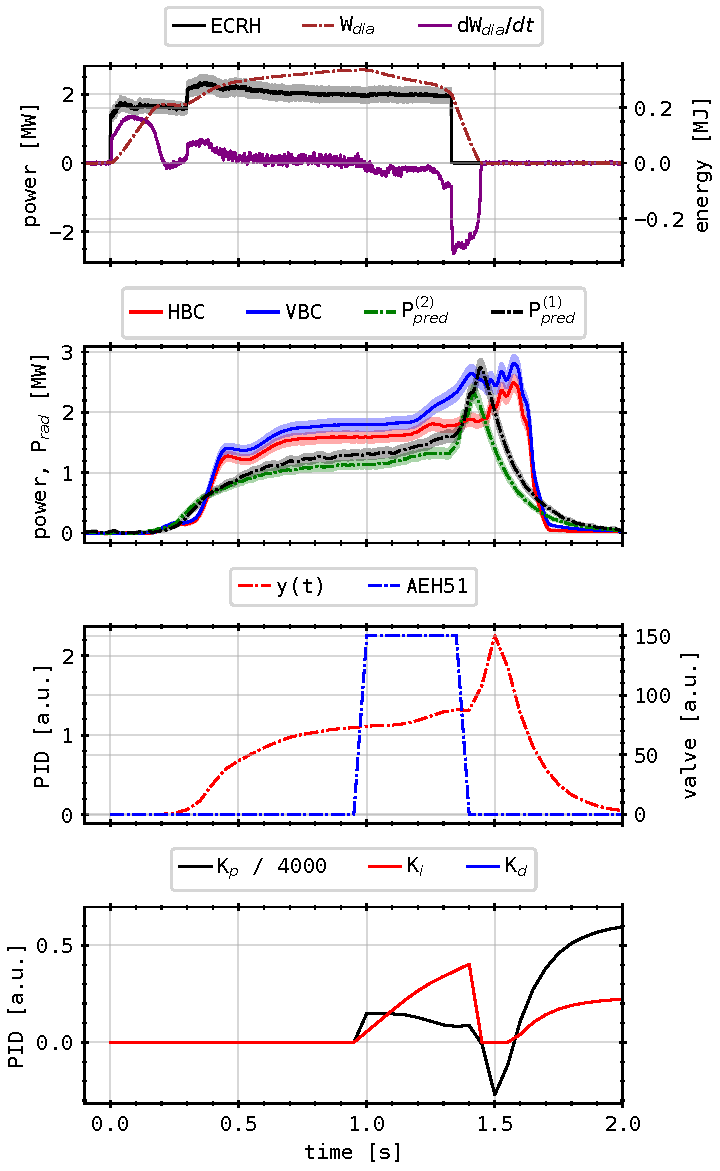
\includegraphics[width=\textwidth]{%
                        content/figures/chapter2/%
                        20180920_029/20180920_029_power_feedback.pdf}%
                \end{subfigure}
                %\hspace*{0.5cm}%
                \begin{subfigure}{0.49\textwidth}%
                    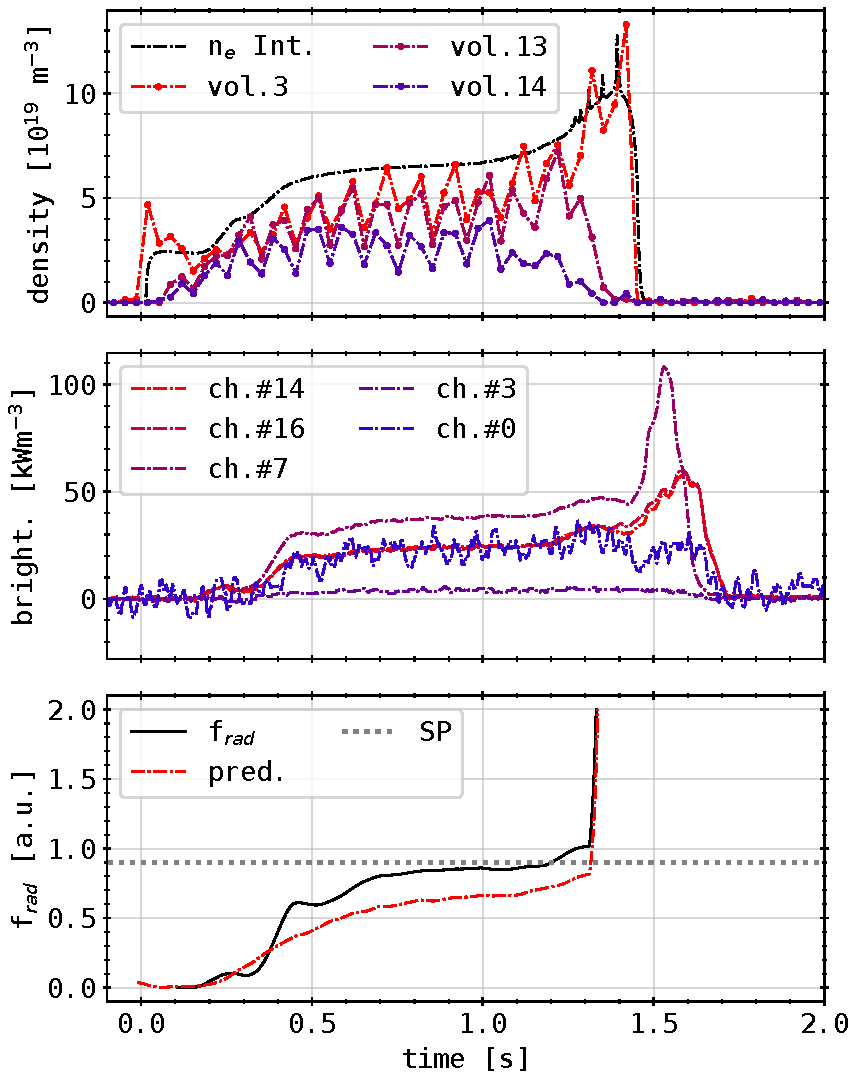
\includegraphics[width=\textwidth]{%
                        content/figures/chapter2/%
                        20180920_029/20180920_029_dens_chord.pdf}%
                \end{subfigure}%
                \caption{%
                    XP20180929.29\\%
                    Very first radiation feedback controlled plasma discharge. \textbf{(top left)}: Microwave heating power, plasma stored energy and loss \textbf{(center left top)}: Radiative power loss, both cameras and prediction values \textbf{(center left bottom)}: PID control $u\left(t\right)$, reference $r\left(t\right)$ and valve actuation \textbf{(left bottom)}: Control components \textbf{(top right)}: Electron density of selected Thomson scattering volumes and line integrated ECE measurement \textbf{(center right)}: Individual bolometer channels, used for $P\ix{pred}^{\left(n\right)}$ \textbf{(bottom right)}: Radiation fraction(s).}\label{fig:20180920.29_PDF}%
            \end{figure}%
%
            The temporal evolution of available plasma parameters can be seen in \cref{fig:20180920.29_PDF}. In the top left, the input heating power and plasma stored energy, as well as its derivative can be found. Below, the total radiative power loss from the plasma, measured by both bolometer cameras can be seen. The real-time radiation $P\ix{rad}$ estimates, calculated by \cref{eq:prediction} and \ref{eq:prediction2} are shown in the same plot. The prediction for $P\ix{rad}$ in $P\ix{pred}^{\left(1\right)}$ was calculated using the detector subset $S=\left\{0, 3, 7, 14, 16\right\}$, as well as the approximation $P\ix{pred}^{\left(2\right)}=a_{7}\Delta\widetilde{U}_{7}$ with detector $7$. This line of sight selection can be seen in \cref{fig:20180920.29_channels}. Below, the PID controls process value $u\left(t\right)$, the forward model $P\ix{pred}^{\left(1\right)}$ for comparison and the normalized feedback valve actuation are presented. Only valves located in port AEH31 injected hydrogen into the scraper-off layer. On the bottom left, the PID components $K\ix{p}$ and $K\ix{i}$ can be seen. No differential component was used in this case. The line integrated electron density from the dispersion interferometer and \textit{Thomson scattering} for selected volumes $\left\{3, 13, 14\right\}$ is shown in the top right. Below, the chord brightness evolution of the bolometer channel subset is presented. Finally, the radiation fraction $f\ix{rad}$, given by \cref{eq:fraction}, next to the setpoint SP of the controller can be seen on the bottom right.\\%
            Both plasma radiation power loss predictions quantitatively roughly mimic the complete $P\ix{rad}$ dataset. Although, the VBC presents a larger $P\ix{rad}$ of at least $10\%$ than the HBC, while the latter shows radiation power values of up to \SI{0.5}{\mega\watt} larger than the predictions. In situations of peak radiation, the proxies $P\ix{pred}^{\left(n\right)}$ are able to represent the full dataset results within their respective error bars. The individual chord brightness of the channels used to calculate the predictions show the same behaviour. However, their temporal relation, i.e. the position of the peak before and after \SI{1.5}{\second} varies significantly. Channel no.7 is maximum at \SI{1.55}{\second}, while detectors viewing plasma volumes further inside with smaller $r_{\text{eff}, M}$, no.14 and 16, reach their peak about \SI{0.1}{\second} later. Due to its orders of magnitude larger noise $\sigma_{\Delta U}$, channel no.0 has no meaningful contribution to the radiation prediction and must have experienced issues during data acquisition. Channel no.3 already shows very small values and therefore suggests no.0 not containing any more information on the emissivity profile, since the chord brightness indicates that the radiation is mainly located inside the last closed flux surface, which will be discussed further below with \cref{fig:20180920.29_CP}. Similar behaviour can be seen in the Thomson scattering electron density for three different volumes - the volumes are ordered so that vol.0 is located closest to the magnetic axis or center of the plasma and vol.16 the furthest away. The line integrated measurement of the dispersion interferometry envelops the lines of the Thomson profile, leading up to the same maximum. The plasma stored energy's derivative indicates that almost all the heating power is deposited into the plasma. However, probes dedicated to measuring the shine-through of the microwaves through the plasma show that there is a non-negligible portion of the heating power beam which is not absorbed.\\%
            % The contributions of $K\ix{p}$ and $K\ix{i}$ to the actuator control can be seen on the bottom left of \cref{fig:20180920.29_PDF}. According to the PV, the valve is opened and closed for injecting hydrogen into the plasma, as is indicated by the actuation of the gas valves. The injection box is located in the diagnostic port AEH51, in the half module of the plasma vessel next to the bolometer measurement plane in counter-clockwise direction. In terms of transport along magnetic field lines, the actuator is one full toroidal rotation away from the bolometer cameras. Due to the delayed response of $P\ix{rad}$ and $P\ix{pred}^{\left(1\right)}$, the control function $u\left(t\right)$ triggers the gas injection early. One gas injection is triggered for \SI{0.35}{\second} after \SI{1.0}{\second}.\\%
%
            \begin{figure}[t]%
                \centering%
                \includegraphics[width=1.\textwidth]{%
                    content/figures/chapter2/20180920_029/%
                    20180920_029_chord_contour.pdf}\\%
                \includegraphics[width=.9\textwidth]{%
                    content/figures/chapter2/20180920_029/%
                    20180920_029_chord.pdf}\\%
                \caption{%
                    XP20180920.29\\%
                    Chord brightness profiles \textbf{(top)} in two-dimensional contours and \textbf{(bottom)} at significant points in time for both cameras HBC and VBC.}\label{fig:20180920.29_CP}%
            \end{figure}%
%
            \autoref{fig:20180920.29_CP} presents the (top) spatial-temporal resolved chord brightness profiles of the horizontal (left) and vertical (right) bolometer camera, as well as (bottom) selected snapshots of the above profiles for both. The radiation, as measured by the HBC, is mainly located inside the projected last closed flux surface, i.e. $r\ix{eff}\in\left\{-1, 1\right\}$ in the chord brightness plot. Similar results are found with the VBC chord brightness profile. Due to the asymmetric line of sight geometry of the vertical camera relative to the magnetic axis, the spatial range is slightly shifted towards the negative, which corresponds to the inside of the vessel or left of the triangular cross-section. The VBC profile features a stronger hollowness of about $50\%$. Furthermore, the small asymmetry of the HBC chord profile is much more pronounced in the vertical camera. The exemplary snapshots of the profile underline this circumstance.\\%
            Due to the delayed response of plasma radiation and therefore difference to the setpoint, the controller engages and initiates two, separate gas inlets. One small and large dent in the radiation power can be found following the actuation of the gas valve and ionization of hydrogen in the scrape-off layer. The radiation power increases accordingly after the first gas injection and step in ECRH around \SI{0.3}{\second}, which leads to $f\ix{rad}\approx 80\%$. However, due to the discrepancy between prediction and full dataset, the PID is assuming a much smaller radiation power, as shown by the red line in \cref{fig:20180920.29_PDF}:(bottom right). The gas valves are opened again, since $P\ix{rad}$ plateaued and has not yet reached the setpoint. The following \SI{0.35}{\second} long hydrogen puff after \SI{1.0}{\second} first slowly increases $P\ix{rad}$ until the \textit{actual} radiation power crosses $f\ix{rad}=90\%$, where it again gains significantly beyond $95\%$. During that time, the electron plasma density collapses from the outside inwards, as at \SI{1.3}{\second} vol.14 is close to zero and vol.13 decreases about $50\%$. Meanwhile, vol.3, i.e. the core plasma, and central line integrated density reach their peak. At this point, the plasma became nearly transparent for the microwave beam and the discharge had to be terminated early.\\%
            Due to the underrepresentation of the \textit{true} plasma radiation power through the prediction $P\ix{pred}^{\left(1\right)}$, the resulting feedback gas puffs increase the actual $P\ix{rad}$ beyond a sustainable level and thereby remove energy by radiative cooling from not only the scrape-off layer, but also the core plasma. Because of the radially shrinking density and temperature profiles, which changes the gradients, the injected hydrogen is transported inside the last closed flux surface and into the confinement regions core plasma. After \SI{1.0}{\second}, the plasma continuously loses $\approx\SI{0.25}{\mega\joule}$ per second, or irradiates \SI{0.25}{\mega\watt}. At increasing density and declining plasma energy, the temperature is assumed to be strongly reduced. The previously discussed radiation asymmetries in chord brightness profiles of both cameras in \cref{fig:20180920.29_CP} can be identified as the connected plasma volume of gas injection (see \cref{fig:divertors_fluxtubes}). Once these profile changes have reduced the absorption of the microwaves enough, the ECRH has to be terminated in order to avoid too much stray radiation on plasma facing components. The remaining \SI{0.2}{\mega\joule} of plasma stored energy are exhausted over the next \SI{0.1}{\second} at nearly \SI{2}{\mega\watt}. This energy is partially irradiated, as $P\ix{rad}$ increases by $\approx\SI{0.75}{\mega\watt}$. The remaining injected hydrogen also dissipates energy by ionization and excitation in the core. The increasing core plasma density quickly drops, as the diamagnetic energy becomes zero and the remaining ionized gas neutralizes. The subsequent final radiation peak at \SI{1.5}{\second} is the result of the residual plasma and its recombination of hydrogen and impurities.\\%
            The radiation feedback XP20180920.29 has failed - by the standards of the in the beginning set-out goals -, since $P\ix{pred}^{\left(1\right)}$ did not provide the required accuracy for an approximation of $P\ix{rad}$ and the system was seemingly not able to achieve a scenario of (stable) detachment. This led to an overshoot of the  density, which caused plasma profiles to collapse and thus the discharge to be terminated earlier than expected. Critical towards the efficiency of the feedback as well is the temporal delay between bolometer detector reaction and valve actuation, albeit it is at this point not quite clear why that is observed here - possible candidates are (impurity) transport physics or intrinsic detector latency. From the chord brightness profile of the vertical and horizontal camera array, the radiation is found to be mainly located close the last closed flux surface, inside the confinement area given the projected LOS $r\ix{eff}$. Therefore, additionally to excluding channel no.0, which was unexpectedly out of order in this experiment, the selection subset $S$ has to be optimized towards this kind of plasma radiation profile. More lines of sight along this radial range have to be included, while channels that do not see any or only small amounts of radiation have be removed from the feedback. However, in order to adequately represent any possible emissivity distribution for varying experiment scenarios, the subset $S$ needs to contain detectors with lines of sight in all plasma regions.%
%
        \subsubsection*{Application Progress}%
%
            The second application of the radiation feedback occurred in experiment XP20180920.31. Regarding the boronisation, the influx of impurities from the wall and general machine condition are assumed to be same as in the previous experiment. This discharge was also planned with \SI{29.5}{\mega\joule} of total input energy at \SI{10}{\mega\watt} X2-mode microwave heating for \SI{10}{\second} in a similarly pre-fuelled hydrogen plasma. Furthermore, the $P\ix{rad}$ proxy settings used for real-time feedback are the same as in experiment XP20180920.29, i.e. $S=\left\{0, 3, 7, 14, 16\right\}$ and $P\ix{pred}^{\left(2\right)}=a_{7}\Delta\widetilde{U}_{7}$, or as in \cref{fig:20180920.29_channels}. Injection is performed from the same valves and port as before, in half module no.5 by AEH51. The net toroidal current increased over the course of the discharge to $\approx\SI{2}{\kilo\ampere}$ in counter-clockwise direction. One important change in this feedback experiment is the integration of a $k\ix{p}=f\left(e\left(t\right)\right)$ so that $K\ix{p}=k\ix{p}=f\left(e\left(t\right)\right)e\left(t\right)$ for the proportional component of the PID activation.\\%
%
            \begin{figure}[t]%
                \centering%
                \begin{subfigure}{.48\textwidth}%
                    \centering%
                    \includegraphics[width=\textwidth]{%
                        content/figures/chapter2/%
                        20180920_031/20180920_031_power_feedback.pdf}%
                \end{subfigure}%
                \hspace*{0.2cm}%\hfill%
                \begin{subfigure}{.48\textwidth}%
                    \centering%
                    \includegraphics[width=\textwidth]{%
                        content/figures/chapter2/%
                        20180920_031/20180920_031_dens_chord_frad_div.pdf}%
                \end{subfigure}%
                \caption{%
                    XP20180929.31: %
                    \textbf{(top left)}: ECRH power, plasma energy and loss \textbf{(center left top)}: $P\ix{rad}$, prediction values \textbf{(center left bottom)}: PID control $u\left(t\right)$, reference $y\left(t\right)$ and valve actuation \textbf{(bottom left)}: Control component(s) \textbf{(top right)}: Electron density of Thomson scattering and dispersion interferometer \textbf{(center right top)}: Electron temperature of Thomson scattering and ECE \textbf{(center right bottom)}: Bolometer channels for $P\ix{pred}^{\left(n\right)}$ \textbf{(bottom right)}: Radiation fraction(s).}\label{fig:20180920.31_PDF}%
            \end{figure}%
%
            The available plasma properties are shown in \cref{fig:20180920.31_PDF}. The structure of the plots is generally the same as for the previous experiment. The duration of the discharge is now \SI{10}{\second}, given by the electron cyclotron heating of $\approx\SI{2.9}{\mega\watt}$. Additionally, the now accessible electron temperature measurements of both the Thomson scattering and electron cyclotron diagnostics are shown in the second plot on the right. The global radiative power loss of both cameras show similar behaviour, though their discrepancy is generally $>10\%$ for most parts of the experiment. Throughout the discharge, the vertical bolometer camera measures significantly more plasma radiation than its horizontal counterpart. The prediction values are similarly related, as $P\ix{pred}^{\left(1\right)}$ indicates about 10\% more radiation power than $P\ix{pred}^{\left(2\right)}$, while the former is as much as 10\% smaller than $P\ix{rad, HBC}$. Differences between the full datasets and predictions are the less pronounced shape of peaks and slopes, smaller gradients in the rise and conclusion of the radiation and a substantial temporal deviation, which can be noticed around the maximums. The chord brightness of the subset that was used to calculate $P\ix{pred}^{\left(1\right)}$ presents the same behaviour as $P\ix{rad}$. As in the previous experiment, the channels further inward, no.14 and no.16 measure overall less radiation power and show smaller response to gas injections than detector no.3, which is viewing close to the separatrix on the inside of the magnetically confined region. Channel no.3 presents the lowest brightness measurement and a negligible reaction to hydrogen seeding. The control $u\ix{PV}\left(t\right)$ here is composed of a proportional and integral part. The underlying system value $y\left(t\right)$, and therefore the prediction, underestimate the radiation level in $P\ix{rad}$ significantly. Initiated actuations of the feedback valve in port AEH51 and subsequent injections of hydrogen precede the peaks in radiation power. The activation of the actuator is dominated by the proportional component of the PID. The potential fifth gas puff is initiated by $K\ix{p}$, as $K\ix{i}$ is surpassed substantially at this point. The leading slopes in actuator signal later in the experiment are supported by an integral component. Width and shape of the peaks in valve opening voltage are dominated by $K\ix{p}$. The electron density $n\ix{e}$ decreases over the course of the discharge to \SIrange[per-mode=reciprocal]{7.5}{4e19}{\per\cubic\meter} from the core further outward. Inversely, the electron plasma temperature is highest after the first ECRH stage at \SI{0.25}{\milli\second} with \SI{5.5}{\kilo\electronvolt} for the innermost Thomson scattering volume. The further outward volumes no.13 and no.14, as well as the ECE measured temperature are significantly lower, well below \SI{1}{\kilo\electronvolt}. After shut-off of heating power, the temperature drops quickly to zero, where large oscillations in Thomson scattering measurements can be found. For very low electron plasma densities, the measurement of temperatures by elastic Thomson scattering is not applicable. Hence, before and after the plasma, those values show very large errors.\\%
%
            \begin{figure}[t]%
                \centering%
                \includegraphics[width=1.\textwidth]{%
                    content/figures/chapter2/20180920_031/%
                    20180920_031_chord_contour.pdf}\\%
                \includegraphics[width=.9\textwidth]{%
                    content/figures/chapter2/20180920_031/%
                    20180920_031_chord.pdf}\\%
                \caption{%
                    XP20180929.31\\%
                    Chord brightness profiles. \textbf{(top)} Two-dimensional contours \textbf{(bottom)} snapshots for both cameras, HBC and VBC around feedback gas puff.}\label{fig:20180920.31_CP}%
            \end{figure}%
%
            The full chord brightness profile of the HBC and VBC, as well as snapshots from before, during and after the first hydrogen gas injection are shown in \cref{fig:20180920.31_CP}. From the perspective of the HBC, the radiation is mainly located inside $r\in\left\{-1, 1\right\}$ as projected from the LOS, with a strong up/down asymmetry. The emission level on the bottom of the triangular cross-section, inside the separatrix and close to the VBC aperture, is at least twofold of that on the top. The \textit{actual} and predicted radiation fraction, based on $P\ix{rad}$ and $P\ix{pred}^{\left(1\right)}$ respectively, differ significantly. At most times, and especially during and after gas injections, the prediction underestimates the actual radiation fraction by at least 10\%. The conservatively set $K\ix{i}$ was not able to affect and achieve a consistently higher radiation fraction by injecting more hydrogen into the scrape-off layer. For a factor of ten larger $K\ix{i}$, the process value $u\ix{PV}\left(t\right)$ would be dominated by an integral component of error compensation later during the discharge and increase the radiative exhaust. This combination of $K\ix{i}$ and $K\ix{p}$ is unable to maintain a constant, high radiation fraction and hence $P\ix{rad}$, therefore causing oscillations. The large gaps in gas injections, which cause the radiation fraction to decrease significantly in-between valve activations, are basically defined by $K\ix{p}$ amd $K\ix{i}$ in the beginning. This can potentially be bypassed and enhanced by a smaller, conservatively scaled differential component $K\ix{d}$, though with the DAQ and plasma radiation latencys this may be a difficult challenge. The significant drops in $P\ix{rad}$ after each gas puff could be dampened by a similarly proportioned $K\ix{d}$ like the previously constructed $10K\ix{i}$, since the differential component scales $\propto\diff P\ix{pred}^{\left(1\right)}/\diff t$. Experiments incorporating $K\ix{d}$ as optimization have been very difficult to perform and similarly strongly depend on the plasma dynamics. Thus, due to the limited set of feedback applications, they are hard to compare to within the large variety of configurations in W7-X.\\%
            To summarize, this set of proportional and integral PID components $K\ix{p}$ and $K\ix{i}$, without a derivative part $K\ix{d}$, is not able to achieve stable detachment by hydrogen seeding. The deliberate gas injections during this discharge are insufficient in radiatively cooling the scrape-off layer sufficiently to achieve that goal. A positional shift of peak radiation location can be observed in the chord brightness profile during gas injections, although the outermost electron densities and temperatures do not indicate perturbations during those times. At the achieved radiation fraction of $\approx75\%$, an improved particle and radiative power exhaust is expected, which is supported by the increasing $P\ix{rad}$ at relatively stable $W\ix{dia}$ under the assumption of a constant target heat load $P\ix{div}$. The desired, as well as theoretically predicted level of $f\ix{rad}$\cite{Feng2016}, at which a significant inwards shift of radiation and plasma profiles is expected, was not achieved.\\%
            The possibility of feedback, based on a real-time radiation prediction was presented. Latency and accuracy of the proxies, defined in \cref{eq:prediction} and \cref{eq:prediction2} as $P\ix{pred}^{\left(n\right)}$ and calculated by the bolometer system using \autoref{alg:algorithm}, are adequate for the application of hydrogen fueling feedback. A different combination of proportional and integral error compensation $K\ix{p}$ and $K\ix{i}$, or even an entirely new set with a differential contribution $K\ix{d}$ can provide the necessary feedback to achieve the desired $P\ix{rad}$.%
            
            % To support this claim, a \textit{synthetic} PID controller, which was previously applied to the system in \cref{fig:pid_results}, has also been used to find different contributions to the control function $u\ix{PV}$ for achieving the desired 90\% level of radiation fraction for the above experiment. In order to adequately address the plasma scenario, the process value is based on the provided $f\ix{rad,XP}$ through the proxy $P\ix{pred}^{\left(1\right)}$. Two scenarios of PID control are presented: $K\ix{p}$ and $K\ix{i}$ can be adjusted, as well as $K\ix{i}$ and $K\ix{d}$ are optimized for a given $K\ix{p}$ from the experiment. Assuming the system value to be%
%
            % \begin{align}%
            %     y\left(t\right)=\left(1-\mathrel{\hat{f}}\ix{rad}\right)u\ix{PV}\left(t\right)+f\ix{rad,XP}\,\,,\nonumber%
            % \end{align}%
%
            % where $\mathrel{\hat{f}}\ix{rad}$ is used to define the cost or efficiency of the control output towards plasma radiation adjustments. For example, to achieve the results shown in \cref{fig:20180920.31_PID}, $\mathrel{\hat{f}}\ix{rad}=0.5$ or 50\%. This is in line with theoretical predictions of operational detachment scenarios, where higher density scrape-off layers are stable at lower impurity concentrations and higher neutral pressures. Furthermore, the control is given a \SI{0.5}{\second} penalty, as is the case during the actual experiment in order to avoid to early gas feedback and cooling of the plasma.\\%
%
            % \begin{figure}[t]%
            %     \centering%
            %     \includegraphics[width=\textwidth]{%
            %         content/figures/chapter2/%
            %         20180920_031/pid_20180920031_fix.pdf}%
            %     \caption{Adjusted, simulated PID controller response based on $f\ix{rad}$ in XP20180920.31. The impact of the feedback on the radiation fraction was modelled linearly by a cost function around a target $\mathrel{\hat{f}}\ix{rad}$. The setpoint SP is set to 0.9 or 90\%. \textbf{(left)}: The algorithm was allowed to control $K\ix{p}$ and $K\ix{i}$. The ratio is noted above, while their values are shown normalized. \textbf{(right)}: PID control derived $K\ix{i}$ and $K\ix{d}$. The proportional $K\ix{p}$ was taken from the experiment data, as seen in \cref{fig:20180920.29_PDF}.}\label{fig:20180920.31_PID}%
            % \end{figure}%
%
            % In the case of optimized integral and proportional components, $K\ix{p}$ roughly mimics the behaviour that was experienced during the actual experiment. In the beginning \SI{0.5}{\second} of feedback, $K\ix{p}$ shows fast scale oscillations due to numerical artefacts. The response of $K\ix{i}$ is two orders of magnitude larger when compared to the respective quantities in the experiment. The relative level is noted as $K\ix{d}:K\ix{i}=1:2/3$. The integral compensation also starts early, together with the proportional contribution, in contrast to the experiment. The resulting \textit{synthetic} radiation fraction model quickly, after the penalty time, rises to the setpoint of 90\%. The enclosed small steps in $K\ix{p}$, in addition to oscillations in the underlying $f\ix{rad}$ from the experiment, lead to under- and overshooting of the mimic radiation fraction around the setpoint. Beyond \SI{5}{\second}, the integral $K\ix{i}$ has significantly levelled out the process value, which causes $K\ix{p}$ to decrease and become negligible. Remaining peaks therein are subject to the underlying $f\ix{rad,XP}$.\\%
            % For a synthetic PID control, including a $K\ix{p}$ as in the experiment of the modelled after radiation fraction, results also now feature a differential component $K\ix{d}$. The PV increases towards 90\% much slower compared to the previous case. At \SI{5}{\second}, $f\ix{rad}\approx0.9$ is reached with a short plateau, after which $K\ix{i}$ and $K\ix{d}$ are not able to compensate the missing proportional scaling. Due to the consistently larger error, the integral component increases and adds to the existing peak in $f\ix{rad,XP}$ at \SI{9}{\second}. The ratio between the individual contributions therefore also differs significantly, where $K\ix{p}:K\ix{i}:K\ix{d}=1:2/5:3/100$. Larger values of $K\ix{d}$ lead to strong oscillations, since no dampening of the control $u\ix{PV}$ to $y\left(t\right)$ is applied. For an ansatz of%
%
            % \begin{figure}[t]%
            %     \centering%
            %     \includegraphics[width=.6\textwidth]{%
            %         content/figures/chapter2/%
            %         20180920_031/pid_20180920031_fix2.pdf}%
            %     \caption{Simulated PID response based on $f\ix{rad}$ in XP20180920.31 including an ansatz with damping over $N\Delta t$ previous samples. Results are obtained for $\mathrel{\hat{f}}\ix{rad}=0.5$ and $N=17$.}\label{fig:20180920.31_PID2}%
            % \end{figure}%
%
            % \begin{align}%
            %     y\left(t\right)=\left(1-\mathrel{\hat{f}}\ix{rad}\right)\euler^{-\left(t-N\Delta t\right)}u\ix{PV}\left(t\right)+f\ix{rad,XP}\,\,,\nonumber%
            % \end{align}%
%
            % with exponential dampening over $N\in\left(5,20\right)$ samples of length $\Delta t$, results do not improve. Including this model of response, the control in \cref{fig:20180920.31_PID2} does not manage to achieve a constant 90\% radiation fraction within the \SI{10}{\second} experiment duration. Though, the overshooting of the integral part is slightly reduced by a stronger $K\ix{d}$.\\%
            % With this approach, it is possible to model and discuss the impact of latency and response of the plasma with regard to the feedback control $u\ix{PV}\left(t\right)$, as well as to study the influence of potential delays between the feedback process value $y\left(t\right)=P\ix{pred}^{\left(1\right)}$ on the \textit{actual} radiation fraction. This is however not within the scope of this work and not further elaborated on.%
%
        \subsection{Radiation Feedback Controlled Discharge}\label{subsec:primew7xfeedback}%
%
            % Radiation feedback controlled discharge at W7-X.%
            The previously discussed real-time radiation feedback experiments were not able to achieve stable, controlled plasma detachment. However, the experimental results and control data indicate that optimizations of the feedback system and scenario may lead to controlled detachment. It was shown that the previous attempts of radiation feedback have performed suboptimally, be it due to the large latency of the valve actuation and plasma response, particular set of $K\ix{x}$ or unoptimized channel selection for $P\ix{pred, n}$. An experiment with a radiation fraction $f\ix{rad}\ge90\%$ and a significant reduction of target heat loads, involving the injection of hydrogen into the scrape-off layer based on real-time approximations of the radiative power loss will be discussed hereafter.\\%
            The experimental data can be seen in \cref{fig:20181010.32_PDF}. Discharge number XP20181010.32 consisted of \SI{9.2}{\second} of plasma with maximum \SI{6.23}{\mega\watt} of electron cyclotron heating power and total input energy of \SI{55}{\mega\joule}. This plasma was heated by microwave radiation coupling to the second-harmonic ordinary (O2-) mode. The plasma vessel was pre-filled by five, \SI{5}{\milli\second} gas puffs of hydrogen at $\approx\SI{200}{\milli\bar\liter\per\second}$. The fast thermal gas injection system also seeded hydrogen at \SI{750}{\milli\bar} into the scrape-off layer. The responsible gas injection valves are the same as in the previously presented experiment. However, the net toroidal current increased to $\approx\SI{0.9}{\kilo\ampere}$ over the course of the discharge in counter-clockwise direction.\\%
%
            \begin{figure}[t]%
                \centering%
                \captionsetup{width=.45\textwidth}%
                \begin{minipage}[c]{0.45\textwidth}%
                    \caption{Line of sight selection for experiment number XP20181010.32, only containing VBC channels. The LOS cones cover all magnetic islands, as well as the core region and parts of the in-between X-points of separatrices.}\label{fig:20181010.32_channels}%
                \end{minipage}%
                \hfill%
                \begin{minipage}[c]{0.5\textwidth}%
                    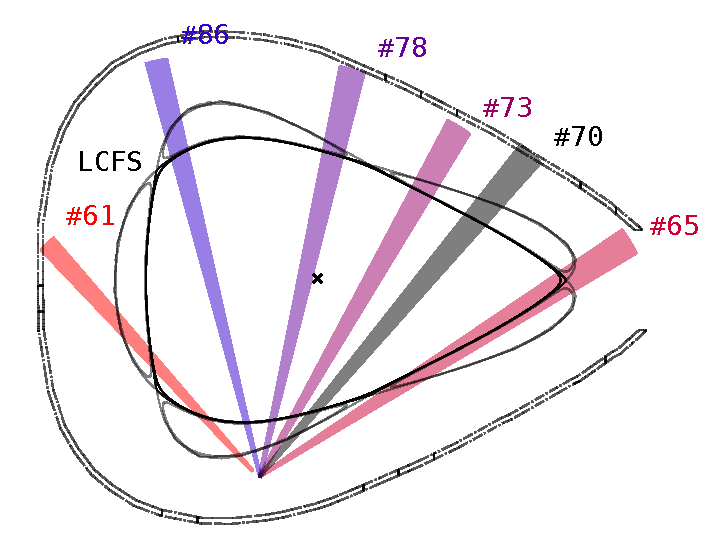
\includegraphics[width=\textwidth]{%
                        content/figures/chapter2/%
                        20181010_032/20181010_32_channels.pdf}%
                \end{minipage}%
            \end{figure}%
%
            In an attempt to provide a more representative radiation power loss proxy for a scenario involving SOL gas injections, the lines of sight selection was changed accordingly. The subset $S=\left\{65, 78, 61, 73, 86\right\}$ was adjusted to consist only of channels from the vertical bolometer camera. The line of sight selection can be seen in \cref{fig:20181010.32_channels}. Previously discussed results showed significant differences between the chord brightness measurements, as well as their toroidal, global power loss extrapolation between the two cameras. The vertical camera, thus far, has seen a greater response of the plasma radiation around the separatrix to the feedback gas injections and overall higher maximum emissivities due to its respective line of sight geometry. Because of the connection along the magnetic field lines between the seeding valves and lower scrape-off layer of the triangular cross-section, the vertical camera is assumed to be more suitable to measuring the impact of gas feedback. So far, the chord brightness indicated the impact of radiation feedback on $P\ix{rad}$ to be largest close to the VBC aperture and around the magnetic islands on the inboard and lower part of the triangular cross-section, where the bolometer is located. The above line of sight selection of vertical camera detectors covers those particular areas, as well as the in-between located X-points, where at very high radiation fractions $f\ix{rad}\rightarrow100\%$ condensation of radiation is expected.\\%
%
            \begin{figure}%
                \centering%
                \begin{subfigure}{.48\textwidth}%
                    \centering%
                    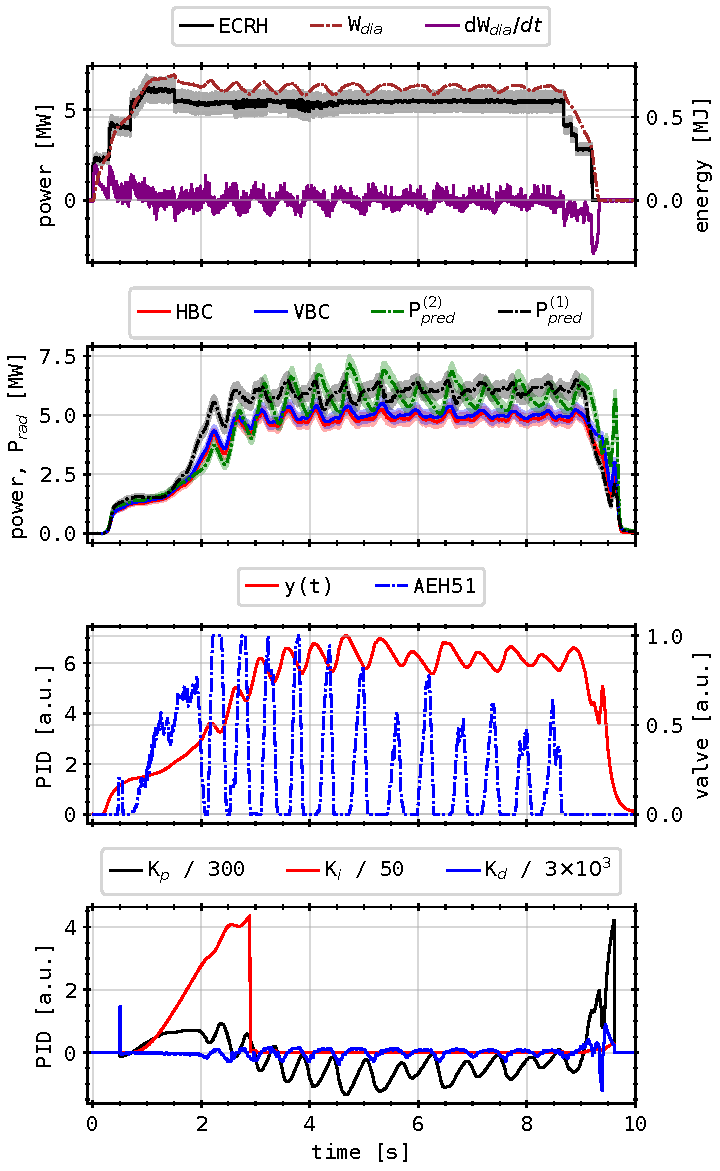
\includegraphics[width=\textwidth]{%
                        content/figures/chapter2/%
                        20181010_032/20181010_032_power_feedback.pdf}%
                \end{subfigure}%
                \hfill%
                \begin{subfigure}{.48\textwidth}%
                    \centering%
                    \includegraphics[width=\textwidth]{%
                        content/figures/chapter2/%
                        20181010_032/20181010_032_dens_chord_frad_div.pdf}%
                \end{subfigure}%
                \caption{%
                    XP20181010.32:\\%
                    \textbf{(top left)}: ECRH power, plasma energy and loss \textbf{(center left top)}: $P\ix{rad}$, prediction values \textbf{(center left bottom)}: PID control $u\left(t\right)$, process value $y\left(t\right)$ and valve actuation \textbf{(bottom left)}: Control components \textbf{(top right)}: Electron density \textbf{(center right top)}: Electron temperature \textbf{(center right bottom)}: Bolometer channels for $P\ix{pred}^{\left(n\right)}$ \textbf{(bottom right)}: Radiation fractions and target heat loads (individual, integrated).}\label{fig:20181010.32_PDF}%
            \end{figure}%
%
            In the data shown in \cref{fig:20181010.32_PDF}, the diamagnetic energy rises gradually, with small changes in slope for each respective ECRH power stage. The level of $W\ix{dia}$ however decreases slightly over the course of the disscharge, on which oscillations of \SI{50}{\kilo\joule} amplitude are superimposed. Those perturbations are in sync with the activation of the gas feedback. The final peak in $\diff W\ix{dia}/\diff t$ after heating is shut off indicates that its initial stages are absorbed with up to \SI{2}{\mega\watt} per increment by the plasma, while the power deposition decreases with increasing plasma energy towards the following microwave power step. \\%
            Within the first two ECRH stages, the radiation power climbs to \SI{1}{\mega\watt}, after which it shortly plateaus and slowly increases to \SI{4.5}{\mega\watt} towards \SI{2.2}{\second}. On top of a slight increment of base level $P\ix{rad}$ to \SI{5}{\mega\watt}, superimposed oscillations as in $W\ix{dia}$ with amplitudes of up to \SI{0.5}{\mega\watt} can be seen. However, these perturbations are \textit{retarded} to the activation of the gas valves, i.e. peaks in $P\ix{rad}$ occur \SIrange{0.2}{0.3}{\second} after the respective gas injection. They also decrease over the course of the discharge. After ECRH shut-off, the radiation power declines sharply, with a conclusive peak due to particle recombinations as the plasma collapses. The horizontal and vertical camera measure a $P\ix{rad}$ that is within their respective error bars, while $P\ix{rad, VBC}$ is consistently larger. Both of the real-time proxies show larger radiation powers than the full camera extrapolations. Before the second oscillation in $P\ix{rad}$ around \SI{3}{second}, the single channel approximation $P\ix{pred}^{\left(2\right)}$, based on a vertical camera channel no.70, indicates smaller values, however with greater perturbation amplitudes afterwards. The subset prediction $P\ix{pred}^{\left(1\right)}$ increases early and presents an up to \SI{1}{\mega\watt} consistently larger radiation power loss. Oscillations therein have slightly smaller amplitudes compared to the other proxy, while both level around \SI{6}{\mega\watt}.\\%
            The control function $u\ix{PV}\left(t\right)$ generally follows the behaviour of the process value $y\left(t\right)$. The gas injection valves are activated when, on the one hand, the overall radiation level as presented by the PV in the beginning is too low, or on the other hand, during falling edges in the oscillations thereof, directly caused by the subsequent gas puffs. At first, during the initial $y\left(t\right)$ plateau, the valves gradually increases gas injection to 75\% of its maximum (solenoid voltage) until \SI{2}{\second}. At this level of activation it is assumed that the valve is opened fully and the gas flow at also maximised. Within the next \SI{2}{\second}, the valve is opened four times fully for $\approx\SI{0.3}{\second}$ each. Afterwards, a similar frequency and duration is maintained at a significantly lower, over time decreasing intensity until \SI{8.75}{\second}. The individual PID components below indicate a dominant proportional and differential contribution $K\ix{p}$ and $K\ix{d}$ for most parts of the feedback. In the beginning however, for the increasing seeding before \SI{2}{\second}, an integral $K\ix{i}$ equally contributes to the actuation of the gas valves. Hence, $K\ix{p}$ and $K\ix{i}$ trigger the system in the beginning, where the radiation level is still low and therefore $f\ix{rad}$ far away from the setpoint: a ramp to \SI{5.5}{\mega\watt} between at \SIrange{0.5}{3}{\second}, followed by a plateau between \SIrange{3}{7}{\second} and finally second ramp from \SIrange{5.5}{6}{\mega\watt} from \SIrange{7}{9.6}{\second}. As soon as $y\left(t\right)$ indicates $>\SI{5}{\mega\watt}$ of radiation power, $K\ix{p}$ and $K\ix{d}$ particularly shape the control function and valve activation. The proportional component is compensating, for one thing, the individual oscillations due to the feedback, and then again a slight increase in process value, which in itself overshoots the setpoint. The significantly faster reaction of the differential $K\ix{d}$ enhances the feedback response to the intrinsic oscillations.\\%
            The presented volumes of the electron density measurement by Thomson scattering have been changed with respect to the previous experiments, though their ordering remains the same. After a steep increase until \SI{1.5}{\second} into a plateau, the electron density of both line integrated interferometer and Thomson scattering measurements show oscillations similar to the ones in $P\ix{rad}$ with varying intensity. The line integrated $n\ix{e}$ goes up to $\approx\SI[per-mode=reciprocal]{1.4e20}{\per\cubic\meter}$ during the on and off of the feedback. From the inside out, the Thomson scattering volumes show descending electron densities of \SI[per-mode=reciprocal]{9e19}{\per\cubic\meter}, \SI[per-mode=reciprocal]{6e19}{\per\cubic\meter}, \SI[per-mode=reciprocal]{3.5e19}{\per\cubic\meter} and \SI[per-mode=reciprocal]{1e19}{\per\cubic\meter} respectively. The further inward volumes no.1 and no.10 increase slightly during and beyond the initial gas injection up to \SI{2}{\second}, however no.14 and no.15 decrease after $P\ix{rad}\approx\SI{3}{\mega\watt}$ around \SI{1.5}{\second}. Line integrated interferometry measurements show sawtooth-like perturbations of the electron densities of \SI[per-mode=reciprocal]{1e19}{\per\cubic\meter} in sync with the actuation of the feedback valves. Thomson scattering volumes no.1 and no.10 indicate no or negligible oscillations. Similar, but less pronounced peaks and drops compared to the interferometry are visible in volumes no.14 and no.15. All densities drop to zero after ECRH shut-off at \SI{9.4}{\second}.\\%
            The electron temperatures are presented for different Thomson scattering, as well as a central electron cyclotron emission volume. A large maximum of \SI{3.4}{\kilo\electronvolt} is found in the first \SI{0.2}{\second} after the start of ECRH. In descending order, this peak is shown by two innermost volumes no.7 and no.1, as well as the ECE core measurement and volume no.10. A further outward electron temperature measurement displays no such peak. By the initial ECRH stages, $T\ix{e}$ increases again after a drop from the previous maximum to up to \SI{3}{\kilo\electronvolt} in the innermost Thomson scattering volume. Number 7, ECE and no.10 respectively show lower electron temperature values down to \SI{0.9}{\kilo\electronvolt}. During the first, longer gas injection, $T\ix{e}$ collectively decreases for all measurement locations, with decreasing impact from the inside outwards. Volume no.10 and no.13 show only very little impact of the radiation feedback, though subsequent perturbations by the valve activations are still noticeable. The ECE and two inner Thomson scattering volumes indicate larger responses to the gas injection of up to \SI{0.4}{\kilo\electronvolt} around their respective average of \SI{0.8}{\kilo\electronvolt}, \SI{2.2}{\kilo\electronvolt} and \SI{1.2}{\kilo\electronvolt}. Further outwards, the electron temperature $T\ix{e}$ in volumes no.10 and no.13 is around \SI{0.6}{\kilo\electronvolt} and \SI{0.2}{\kilo\electronvolt}, with variations of at most \SI{0.1}{\kilo\electronvolt}. These oscillations are anticyclical to the gas injections and radiation power loss measurements, i.e. when $P\ix{rad}$ increases due to a hydrogen puff in the scrape-off layer, the temperatures decrease and vice versa. After \SI{8.5}{\second}, where the ECRH starts to decrease, the electron temperature quickly drops to zero in all locations before \SI{9.5}{\second}.\\%
            The chord brightness of the subset $S=\left\{61, 65, 70, 73, 78, 86\right\}$ for radiation prediction $P\ix{pred}^{\left(1\right)}$ and channel no.70 for $P\ix{pred}^{\left(2\right)}$ largely resemble the already presented $P\ix{rad}$ and aforementioned proxies. The line integrated radiation power density greatly differs among the selected channels and lines of sights. The colour of the plots matches the in \cref{fig:20181010.32_channels} presented lines of sight. Channels no.70, no.86, no.73 and no.78 share a shallower slope than the overall $P\ix{rad}$. They also present similar or slightly larger average emissivities like in XP20180920.31 of \SIrange{80}{160}{\kilo\watt\per\cubic\meter}. A noticeable temporal shift between the aforementioned channels can be seen, i.e. no.70 has peaks where no.78 and no.86 have local minima, while maxima are found later the higher the emissivity. The response to the gas injection is within \SI{40}{\kilo\watt\per\cubic\meter} for those channels during this experiment. The radiation intensities measured by channel no.65 and no.61 greatly differ from the previous ones. Both show a very steep rise during the initial heating stages, with a subsequent plateau and slight decrease until \SI{1.5}{\second}. After, channel no.65 goes up to average $\approx\SI{290}{\kilo\watt\per\cubic\meter}$, with oscillations of up to \SI{60}{\kilo\watt\per\cubic\meter}. Channel no.61 reaches a baseline of \SI{360}{\kilo\watt\per\cubic\meter}, from which perturbations due to the gas injection vary between \SIrange{40}{100}{\kilo\watt\per\cubic\meter} over the course of the discharge. Between \SIrange{4}{5.5}{\second} and around \SI{6.75}{\second}, the peaks and drops in no.61 are extraordinarily larger than during other gas puffs. These oscillations appear retarded to the hydrogen injections by around \SIrange{0.2}{0.3}{\second}. A small increase in baseline of $\approx\SI{40}{\kilo\watt\per\cubic\meter}$ during the cycling of the feedback is also visible in channel no.65 and no.61. Their local maxima and minima occur later than the previous channels, which measure lower emissivities. However, after the ECRH step down at \SI{8.5}{\second}, the radiation intensity starts to decrease first in those channels, before no.73, no.78, no.86 and no.70 peak and sharply drop to zero around \SI{9.5}{\second}.\\%
            The resulting radiation fractions of both the presented proxy $P\ix{pred}^{\left(1\right)}$ and mean between $P\ix{rad,HBC}$ and $P\ix{rad,VBC}$ are shown next to the heat load of the individual divertors and the integrated $P\ix{div}$. Both proxy and $P\ix{rad}$ show an overall similar behaviour of $f\ix{rad}$, though, as seen before in $P\ix{pred}^{\left(1\right)}$, the total radiation power loss is being overestimated by the prediction, which leads to a larger and even greater than unity ($P\ix{rad}>P\ix{ECRH}$) radiation fraction. During the initial stages in microwave heating, $f\ix{rad}$ quickly increases to 30-40\%, before dropping again after the final ECRH power is reached. By the first, longer gas injection, the radiation fraction goes up to 80\%. Subsequent valve actuations increase $f\ix{rad}>90\%$ towards \SI{3.5}{\second}. For the power loss derived from the mean $P\ix{rad}$ of both camera arrays, the following gas puffs cycle the radiation fraction between 90\%-100\%. Towards the end of the experiment, i.e. \SI{9}{\second}, the perturbation amplitude decreases and the mean $f\ix{rad}\rightarrow90\%$ due to compensations in control $u\ix{PV}\left(t\right)$ and reduced gas injection. Since $y\left(t\right)=P\ix{pred}^{\left(1\right)}$ and the prediction overestimates $P\ix{rad}$, the radiation fraction provided to the feedback control is significantly larger than 100\% during the alternation of the valve control. In accordance to $P\ix{rad}$ and the adjustments in gas injection, the perturbations in $f\ix{rad}$ decrease over time, where in the beginning variations of up to 15\% can be seen. From prediction $P\ix{pred}^{\left(1\right)}$, $f\ix{rad}$ even reaches 120\% and oscillates between 115-105\%. The integrated target heat load increases quickly until the maximum microwave heating is achieved at $\approx\SI{1}{\second}$ to \SI{4.2}{\mega\watt}. Afterwards, by the initial long and subsequent shorter hydrogen injections, $P\ix{div}$ decreases to \SI{2}{\mega\watt} at first and then averages around \SI{1.4}{\mega\watt} over the following gas puffs. Similar to $P\ix{rad}$, the response in target heat load to the later valve actuations decreases towards \SI{8.5}{\second}. After the final gas puff, $P\ix{div}$ decreases to \SI{0.8}{\mega\watt}, from which it drops to zero at \SI{9.3}{\second}. The heat load of the individual targets is largely symmetrically distributed. However, the divertors HM51 and HM10 indicate a non-negligible, larger thermal power of \SIrange{50}{100}{\kilo\watt}, or 20-40\% more than the other modules. In direction of the counter-clockwise, net toroidal plasma current, the targets HM51 and HM10 in the respective half modules no.5 and no.1 are connected with each other by parallel transport along field lines. Furthermore, with respect to \cref{fig:divertors_fluxtubes}, this also connects to the responsible gas valves in module HM51, as well as the lower and inside magnetic islands.\\%
%
            \begin{figure}[t]%
                \centering%
                \includegraphics[width=1.\textwidth]{%
                    content/figures/chapter2/20181010_032/%
                    20181010_032_chord_contour.pdf}\\%
                \includegraphics[width=.9\textwidth]{%
                    content/figures/chapter2/20181010_032/%
                    20181010_032_chord2.pdf}\\%
                \caption{%
                    XP20181010.32\\%
                    Chord brightness profiles. \textbf{(top)} Two-dimensional contours \textbf{(bottom)} snapshots for both cameras, HBC and VBC around feedback gas puff.}\label{fig:20181010.32_CP}%
            \end{figure}%
%
            In \cref{fig:20181010.32_CP} the chord brightness profiles of both vertical and horizontal camera, as well as temporal snapshots around one hydrogen gas puff at $f\ix{rad}\approx90\%$ can be seen. Similar to the previous experiment, the majority of emissivity is located at or around $r\ix{eff}=\pm r\ix{a}$. The poloidal asymmetry in chord brightness as measured by the HBC is reversed compared to before, with local maxima being strongly radially focused at the separatrix $r\ix{eff}/r\ix{a}=1$. For each of the gas puffs and subsequent peaks in $P\ix{rad}$, a concurrent peak in the chord brightness profile with an overall radial inward shift of emissivity can be found. The temporal snapshots emphasize the (radial) asymmetry during gas injections, as well as show the evolution of the maximum emissivity at the separatrix $r\ix{eff}=r\ix{a}$. At $-r\ix{a}$, the emissivity increases from \SIrange{80}{380}{\kilo\watt\per\cubic\meter} for one hydrogen injection. The small inward shift is visible in the peak position on the negative end of the radial spectrum. The absolute maximum is located opposite of the peaks that have been measured during the previous experiments. The responsible lines of sight cover areas that are opposite to the aperture of the VBC and do not overlap with the magnetic island on the inboard side. The chord brightness of the vertical camera now shows a small poloidal asymmetry, which is supported by the individual profiles below. Local maxima can be found around the separatrix at $r\ix{eff}=-r\ix{a}$ after gas injections, with parallel inward shifts of the radiation on both sides of the profile. As in the top of the HBC chord brightness, the radial gradients are much stronger on the bottom of the vertical camera profile. In addition, there is a significant gap in the radial evolution of the emissivity on the inside of the separatrix of the inboard side. In comparison to the peak evolution for a single gas puff in the horizontal profile, the vertical camera measures only an increase of $\approx33\%$ around $-r\ix{a}$.\\%
            The resulting power balance for this discharge can be seen in \cref{fig:20181010.32_balance}. Within the first \SI{2}{\second} $P\ix{bal}=0$ is satisfied inside its error bars, though the individual lines for $P\ix{rad}$ indicate an underestimation of losses of $\approx\SI{1}{\mega\watt}$. After the first gas injection, the power balance starts to oscillate with the individual gas puffs, as seen in the radiation power loss $P\ix{rad}$, plasma energy $W\ix{dia}$ and its derivative, as well as the divertor heat load $P\ix{div}$. On average, $P\ix{bal}$ indicates a significant overestimation of the cumulative power losses of $\approx\SI{1.5}{\mega\watt}$. Perturbations due to the feedback injections cycle around this level by about \SI{1}{\mega\watt}, with decreasing impact of each gas puff towards the end of the discharge. Due to the large error bar of $\approx\SI{0.8}{\mega\watt}$, the power balance can be assumed to be occasionally off by only \SI{0.3}{\mega\watt} following individual valve activations. After the ECRH starts to step down, $P\ix{bal}$ declines in two drops due to the collapse of the plasma and dissipation of the stored energy to $\-\SI{2.5}{\mega\watt}$ and $\-\SI{4}{\mega\watt}$.\\%
%
            \begin{figure}[t]%
                \centering%
                \includegraphics[width=0.6\textwidth]{%
                    content/figures/chapter2/%
                    20181010_032/20181010_032_power_balance.pdf}%
                \caption{XP20181010.32\\%
                    Power balance for both $P\ix{rad}$ of the individual camera arrays and a (grey) mean with error bar, derived from the intrinsic errors of the contributing physical quantities.}\label{fig:20181010.32_balance}%
            \end{figure}%
%
            The measurement data of this experiment presents evidence of \textit{feedback controlled stable plasma detachment}. Hydrogen gas injection into the scrape-off layer, controlled by real-time radiation power loss measurements was able to achieve and maintain a radiation fraction $f\ix{prad}>90\%$ for extended durations. Its application raises the overall radiation level, as well as significantly increases the emissivity along and close to the magnetic separatrix. The achievement of $f\ix{rad}\ge70\%$ is accompanied by an inward shift of radiation towards the separatrix and center of the confined region. This is supported by the fact that the response to the individual gas puffs is, on the one hand, varying strongly in amplitude across the chord brightness profile, and on the other, temporally retarded with respect to different parts of the profile and their respective peaks and drops. The chord brightness profiles suggest radiation condensation, after increasing the radiation fraction $>80\%$, in the inboard magnetic island and X-points towards the neighbouring islands on the top and bottom of the triangular cross-section. Therefore, the lines of sights covering those areas measure factor two to three larger emissivities compared to detectors mainly viewing the magnetically confined region. The magnetic island located on the inboard side is connected to the responsible feedback valves in half module no.5 (AEH51) by the plasma transport along field lines. The focussing of radiation power loss at X-points and close to the separatrix, i.e. in magnetic islands at significantly higher $f\ix{rad}>70\%$, was predicted by results from the similarly configured W7-AS experiment and simulations of impurity radiation using EMC3-EIRENE\cite{Feng2005,Thomsen2004,Feng2016}. In addition, there is no degradation of the plasma stored energy, as $W\ix{dia}$ only increases until $f\ix{rad}>80\%$ and only small perturbations of the overall level due to individual gas injections can be found. The line integrated electron density presents similar behaviour, where $n\ix{e}$ starts to plateau at $f\ix{rad}\approx80\%$ and then slightly increases over the subsequent hydrogen injections. Individual Thomson scattering volumes close to the magnetic axis indicate smaller densities, though with comparable development as the line integrated density at lower values. No concurrent perturbations due to the gas puffs can be seen. The two outermost scattering volumes indicate a drop following their initial increase after the radiation fraction reaches 40\%. They present, in contrast to the volumes further inwards, significant perturbations due the gas injections, which are anticyclical to $f\ix{rad}$. The electron density close to the separatrix inside the confined area decreases $\approx30\%$ when the radiation fraction goes from 90\% to 100\% and vice versa. Contrary, the electron temperature measured in the innermost volumes and from cyclotron emissions presents inverse behaviour to $f\ix{rad}$, while volumes further towards the separatrix display negligible interference by hydrogen injections. Also, the prior similarly drop from their respective maximum after $f\ix{rad}>40\%$. Towards high radiation fractions $f\ix{rad}>70\%$, a significant decrease of the plasma density close to the separatrix is expected, which leads to a steepening of the profile. For $f\ix{rad}\approx90-100\%$ the perturbations in volumes closer to the separatrix, opposite to changes in radiation fraction, indicate the inward shift of the plasma and therefore reduction of perpendicular transport to the scrape-off layer. However, in this case the accompanying temperature distribution flattens and only changes significantly closer to the magnetic axis. Though, assuming constant temperature profiles close to the separatrix, the net perpendicular plasma flux across field lines is reduced due to smaller gradients and the decreased density. Lastly, the integrated divertor heat load supports the previous arguments. After the radiation fraction increases beyond 40\%, $P\ix{div}$ decreases with increasing $f\ix{rad}$ until it is more than halved at $f\ix{rad}\approx80\%$. With each subsequent gas injection and peak to 100\% radiation fraction, the target heat load decreases further, before receding again with the concurrent drop in $f\ix{rad}$. The significantly larger heat loads of divertor modules HM51 and HM10 suggest a substantial contribution of the plasma radiation to the incident power of plasma target components in scenarios with very high $f\ix{rad}$ and controlled radiative cooling in neighbouring plasma volumes. In this particular case, the parallel transport along field lines directly links the aforementioned modules, feedback gas valves and, indirectly in the second to next half module, inboard magnetic island in the bolometer measurement plane. The chord brightness reflects this as well, where the emissivity is twofold of that on the opposite side of the profile and at \SI{400}{\kilo\watt\per\cubic\meter} extraordinarily high when compared to the previous experiments.\\%
            In conclusion, this radiation feedback controlled experiment has achieved \textit{stable plasma detachment} by gas injections into the scrape-off layer. The target heat load was significantly reduced by a factor of over two, while a radiation fraction and therefore radiative power loss $>90\%$ of the input heating power was maintained by the PID controlled feedback system. During the gas injection, neither degradation of the plasma stored energy nor the core electron density, i.e. close to the magnetic axis, was found. However, the evolution of the electron temperature profile in its entirety indicates a stronger coupling to the radiation fraction than the electron density. A small but noticeable inward shift of the radiation distribution profile is measured by both bolometer cameras. The feedback control is able to consistently increase the radiation fraction $>80\%$ by controlled injection of hydrogen, in this case the working gas. In succession to reaching $f\ix{rad}\approx90\%$, the feedback input underestimates the impact of the individual gas injections, which leads to strong oscillations in $P\ix{rad}$ of up to 10\% of the heating power for full activation of the valves. Towards the end of the experiment however, the PIDs differential component can steadily reduce the overshooting of the control and therefore reduce the oscillations in $P\ix{rad}$ and conclusively $f\ix{rad}$. Another significant factor to the cycling of PID control and valve activation is the latency of the feedback prediction and response of the plasma to the injections. Although the radiative power loss proxy $P\ix{pred}^{\left(1\right)}$ is consistently larger than $P\ix{rad}$ from either cameras' measurement, the adjusted channel selection $S$ in \cref{fig:20181010.32_channels}, consisting of detectors from the vertical camera arrays viewing the magnetic islands and X-points, has improved the quality of the feedback.\\%
            It should be noted that the PID parameters and $K\ix{i}$ in particular were not optimized towards a steady-state performance here with respect to the radiation feedback. As pointed out in the beggining, with this being the ultimate goal of the outlined diagnostic setup, such long-term steady-state experiments also with radiation feedback are planned for the future. With this limited set of dicharges, the $K\ix{x}$ could not be improved towards that given the complex entanglement and large combination space of plasma parameters.%
%
        \subsection{Comparison to Feedback Control on Different Physical Quantities}\label{subsec:densityfeedback}%
%
            % Comparison to density feedback control.
            The real-time radiation feedback system was able to perform plasma control based on other properties than the radiative power loss. In \cref{sec:configuration}, the dispersion interferometer, measuring the line integrated electron density, and optical fibre filterscopes, with lines of sight parallel to the horizontal divertors were introduced as additional candidates for plasma detachment control with the thermal helium beam gas valves as an actuator. In order to fully discuss the quality of the radiation feedback and categorize its results, a comparison to the achievements of the different control proxies is imperative.%
%
            \subsubsection*{Electron Density From Dispersion Interferometer}%
%
                Similar to XP20181010.32, which featured controlled detachment by radiation feedback, this example of electron density feedback in experiment number XP20181016.16 consisted of hydrogen gas injections in half module HM51 by the same valves. Measurement results of this pre-filled hydrogen plasma can be seen in \cref{fig:20181016.16_PDF}. A constant \SI{5}{\mega\watt} of O2-mode microwave heating was applied for \SI{21}{\second}, after two initial, smaller steps at \SIrange{3}{4.5}{\mega\watt} within the first \SI{1}{\second}, before decreasing to \SI{4.5}{\mega\watt} for the remaining \SI{9}{\second}. The plasma energy increases with small changes in slope, according to the steps in heating power, to \SI{0.65}{\mega\joule}. After the feedback gas injection starts at \SI{2}{\second}, there is a small drop in $W\ix{dia}$, which is followed by a decline towards \SI{0.6}{\mega\joule} until the step-down in ECRH. This is also reflected in the plasma energy. Besides the initial heating of the plasma and its collapse after \SI{32}{\second}, the plasma power loss $\diff W\ix{dia}/\diff t$ presents high frequency, random perturbations between $\-$\SIrange{0.1}{0.1}{\mega\joule}, which decrease slightly towards the end of the discharge.\\%
%
                \begin{figure}[t]%
                    \centering%
                    \begin{subfigure}{.48\textwidth}%
                        \centering%
                        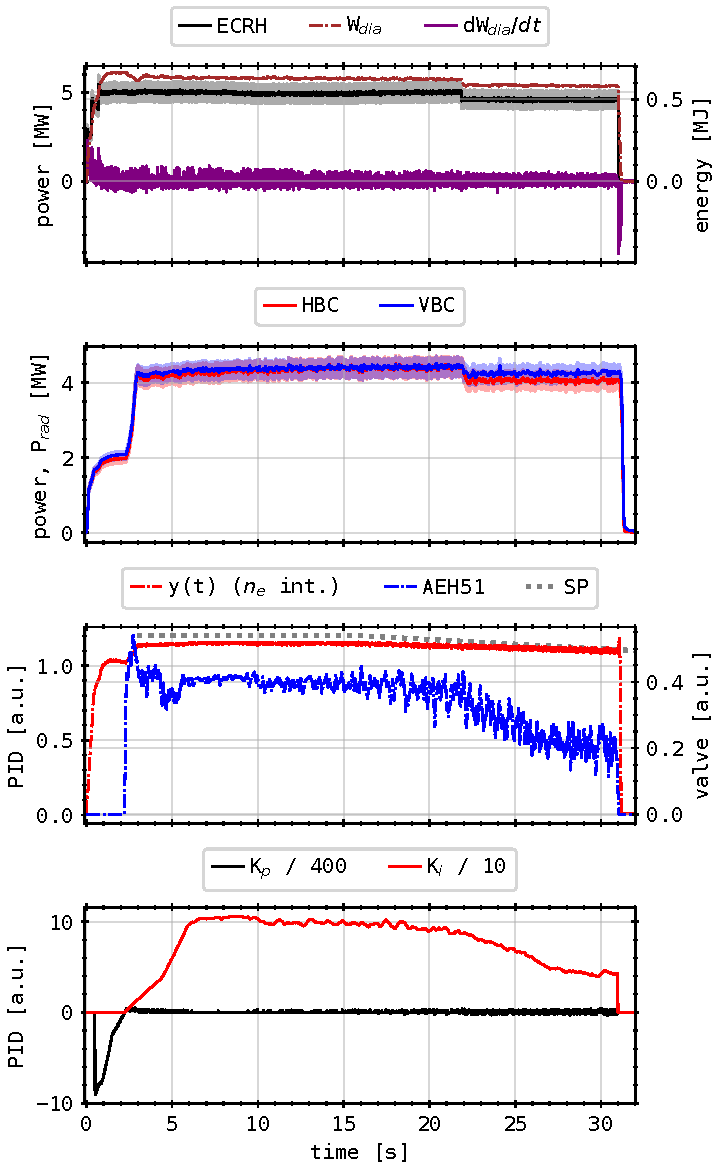
\includegraphics[width=\textwidth]{%
                            content/figures/chapter2/%
                            20181016_016/20181016_016_power_feedback.pdf}%
                    \end{subfigure}%
                    \hfill%
                    \begin{subfigure}{.48\textwidth}%
                        \centering%
                        \includegraphics[width=\textwidth]{%
                            content/figures/chapter2/%
                            20181016_016/20181016_016_dens_chord_frad_div.pdf}%
                    \end{subfigure}%
                    \caption{%
                        XP20181016.16:\\%
                        \textbf{(top left)}: ECRH, plasma energy and loss \textbf{(center left top)}: $P\ix{rad}$ \textbf{(center left bottom)}: Process value $y\left(t\right)$ and valve actuation \textbf{(bottom left)}: Control components \textbf{(top right)}: Electron density \textbf{(center right)}: Electron temperature \textbf{(bottom right)}: Radiation fractions and target heat load.}\label{fig:20181016.16_PDF}%
                \end{figure}%
%
                Radiation power loss $P\ix{rad}$ from both bolometer cameras are within their respective error bars. Following the heating stages in the beginning, $P\ix{rad}$ plateaus around \SI{2}{\mega\watt} before increasing to \SI{4.15}{\mega\watt} after the hydrogen gas feedback starts at \SI{2}{\second}. The radiation power increases $\approx\SI{0.1}{\mega\watt}$ before the step-down in ECRH. Afterwards, $P\ix{rad}$ also steps down with the heating power to \SI{4.05}{\mega\watt}, from which it drops to zero as the plasma collapses after \SI{31.5}{second}.\\%
                The process value and feedback variable of this detachment experiment was the line integrated electron density, which was provided by the dispersion interferometer. A slowly declining $n\ix{e}$ ramp around \SI[per-mode=reciprocal]{1.1e20}{\per\cubic\meter} in the second half of the discharge for this microwave heating and feedback configuration was developed from experiences of previous experiments. The density setpoint for this feedback was designed to achieve a constant, high plasma radiation fraction $f\ix{rad}>90\%$\cite{Krychowiak2021, Krychowiak2023}. Consequently, the proportional PID component $K\ix{p}$ prohibits gas injections before \SI{2}{\second}, as $n\ix{e}$ sharply rises towards its setpoint value. The following gas valves activation is exclusively determined by the integral component $K\ix{i}$. When the downward ramp in density begins, $K\ix{i}$ also decreases similarly to the valve actuation by a factor of two. The subsequent hydrogen gas injection starts at \SI{2}{\second}, which increases $n\ix{e}$ from \SIrange[per-mode=reciprocal]{1}{1.15e20}{\per\cubic\meter}. After \SI{17}{\second}, the electron density declines to \SI[per-mode=reciprocal]{1.08e20}{\per\cubic\meter} toward the end of the discharge. Thomson scattering volumes further inward exhibit similar behaviour, however at lower values and with smaller responses to the hydrogen injection. Volume no.15 shows a decline after \SI{2}{\second} and a stronger ramp down than the line integrated density towards \SI{31}{\second}, while $n\ix{e}$ of inside volumes increases minutely. The electron temperature initially increases quickly to its maximum \SI{2.6}{\kilo\electronvolt} in the innermost Thomson scattering volumes. Afterwards, $T\ix{e}$ declines with the gas feedback and then again with the downward step in heating power. This behaviour is found for all temperature measurements, at lower values further outward and closer to the separatrix. Overall, the average electron temperatures are comparable to measurement results in XP20181010.32.\\%
                The resulting radiation fraction and target power adjust accordingly to the increase in radiation fraction. As the gas injections increase $n\ix{e}$ to its ramp-like setpoint, the divertor heat load $P\ix{div}$ drops by 50\%, while $f\ix{rad}$ rises to 80\% with a small incline to 90\% towards \SI{10}{\second}. Integrated heat load and radiation fraction remain relatively constant throughout the rest of the discharge. Similar to XP20181010.32, two divertor modules in HM51 and HM11, close to the gas valves and along the direction of parallel plasma transport, show significantly larger heat loads in comparison to the others. Also, similar to the radiation feedback detachment, $P\ix{div}$ already starts to decrease substantially as $f\ix{rad}\approx50\%$ and above, as well as $T\ix{e}$ and $n\ix{e}$ of volumes further outward begin to decline.\\%
%
                \begin{figure}[t]%
                    \centering%
                    \includegraphics[width=.6\textwidth]{%
                        content/figures/chapter2/20181016_016/%
                        20181016_016_power_balance.pdf}%
                    \caption{XP20181016.16\\%
                        Power balance for both $P\ix{rad}$ (red, blue) of individual camera arrays and a (grey) mean with error bar.}\label{fig:20181016.16_balance}%
                \end{figure}%
%
                The global power balance for this experiment is shown in \cref{fig:20181016.16_balance}. There is a surplus of \SI{1}{\mega\watt} of heating power in the initial \SI{2.5}{\second}, which is not accounted for in loss terms. After the feedback starts injecting hydrogen, $P\ix{rad}$ increases by over \SI{2}{\mega\watt} and $P\ix{div}$ drops by \SI{1}{\mega\watt}. The resulting power balance adjusts accordingly and indicates $\approx\-\SI{0.2}{\mega\watt}$, while $P\ix{bal}=0$ is satisfied within the error bar. From \SI{20}{\second} and following the step-down in heating power, $P\ix{bal}$ begins to increasingly deviate from zero over time. The individual lines for either cameras $P\ix{rad}$ start to diverge more, with $P\ix{bal}$ from radiative power loss measurements of the horizontal camera being closer to zero than from the vertical.\\%
%
                \begin{figure}[t]%
                    \centering%
                    \includegraphics[width=1.\textwidth]{%
                        content/figures/chapter2/20181016_016/%
                        20181016_016_chord_contour.pdf}%
                    \caption{XP20181016.16: %
                        Chord brightness profile of HBC and VBC.}\label{fig:20181016.16_CP}%
                \end{figure}%
%
                The chord brightness profile for both bolometer cameras can be seen in \cref{fig:20181016.16_CP}. Very similar results to  XP20181010.32 are presented. The HBC measures a strong poloidal asymmetry, with the maximum emissivity on the top of the triangular cross-section throughout the entire discharge. A similar structure on the inside, closer to the magnetic axis, is found for $f\ix{rad}>50\%$. The peaks on both ends of the radial spectrum are located in the same position as before, i.e. $r\ix{eff}=r\ix{a},\,0.8r\ix{a}$. Poloidal asymmetries for $f\ix{rad}>50\%$ in the HBC chord profile decrease towards the step-down in heating power at \SI{22}{\second}. The maximum in brightness shifts to the other side at $r\ix{eff}\approx0.7r\ix{a}$, while the peak on the negative end of the radial spectrum has almost entirely flattened. Vertical camera measurements also present local maxima at $r\ix{eff}=\-r\ix{a},\,0.9r\ix{a}$ for the entire duration of the discharge, with a substantial gap on the inside of the separatrix and negative end of the radial spectrum in the chord brightness. There is no reversal of the local maxima after \SI{22}{\second} in the VBC profile. However, the peak around $\-r\ix{a}$ has decreased significantly to a similar level of the local maximum at $0.8r\ix{a}$. A small inward shift towards the magnetic axis of the chord brightness can be seen. For both cameras profiles, in agreement with the temporal evolution of $P\ix{rad}$ and in contrast to XP20181010.32, there are no oscillations in the profiles due to cycling of gas injections. Furthermore, the total radiative power loss is \SI{0.5}{\mega\watt} lower than the average during the radiation feedback detachment. The maximum chord brightness however is about is up to 20\% and 15\% lower for the horizontal and vertical camera, respectively. With the step-down in heating power at \SI{21.8}{\second}, the chord emissivity also decreases slightly.\\%
                In conclusion, the electron density feedback results in a significant reduction of divertor heat load by radiatively cooling the scrape-off layer and increasing the radiation fraction, like it was discussed for the case of radiation feedback. The gas injection system aims to achieve a high performance plasma in terms of core electron density, which is defined by the previously explored $n\ix{e}$ setpoint at \SI{1.1e20}{\per\cubic\meter}. Additionally, a slow ramp down in electron density is programmed in order to compensate for a gradual increase in $P\ix{rad}$ over time due to a slowly increasing amount of intrinsic impurities. Accordingly, the radiation fraction is well adjusted above 80\%, which leads to the already alluded to shaping of the electron density and temperature profiles. The more direct coupling, with less latency when compared to the radiation feedback, of hydrogen gas injections to the feedback proxy $n\ix{e}$ yields much smoother and reliable results, without oscillations, in target heat load reduction.\\%
                Results from this and the previously discussed feedback experiment and their respective comparison underline the prefixed relation in \cref{eq:lineradiation}, particularly with regards to its dependency in plasma density. A necessary challenge therefore will be the exploration of that parameter space, albeit the character and number of those quantities are not known, especially in the case of plasma feedback.%
%
            \subsubsection*{C-III Radiation From Filterscopes}
%
                The third candidate for plasma feedback control was the C$^{2+}$ (carbon) radiation intensity in front of the target, which is measured by filterscopes. The results of XP20180920.32 can be seen in \cref{fig:20180920.32_PDF}. Like before, hydrogen is seeded into the scrape-off layer of a pre-filled hydrogen plasma by thermal gas injection valves in AEH51. In contrast to the previous experiments, this plasma was heated by microwave radiation coupling to the second-harmonic extraordinary (X2-) mode. After an initial step at \SI{1.5}{\mega\watt}, a constant \SI{3}{\mega\watt} of ECRH was applied to the plasma for \SI{9.5}{\second}. The plasma energy increases to \SI{0.5}{\mega\joule}, from which it declines towards the termination of the discharge. When the gas feedback sets in at \SI{2}{\second}, there appears a small increase in $W\ix{dia}$. Its time derivative reflects this behaviour, as two initial increments in heating power and the plasma collapse at \SI{10}{\second} can be distinguished in $\diff W\ix{dia}/\diff t$.\\%
                Both bolometer cameras measure similarly behaving radiation powers, while the VBC indicates $\approx10\%$ larger values than the HBC. After the start of the ECRH, $P\ix{rad}$ plateaus at \SI{1}{\mega\watt}, with a minor incline slope until \SI{2.5}{\second}. Following the beginning of gas injections, the radiation power loss gradually increases, until slowly equilibrating around \SI{8}{\second} at $\approx\SI{2}{\mega\watt}$. About \SI{0.5}{\second} after the ECRH is shut off, $P\ix{rad}$ drops to zero as the plasma collapses.\\%
%
                \begin{figure}[t]%
                    \centering%
                    \begin{subfigure}{.48\textwidth}%
                        \centering%
                        \includegraphics[width=\textwidth]{%
                            content/figures/chapter2/%
                            20180920_032/20180920_032_power_feedback.pdf}%
                    \end{subfigure}%
                    \hfill%
                    \begin{subfigure}{.48\textwidth}%
                        \centering%
                        \includegraphics[width=\textwidth]{%
                            content/figures/chapter2/%
                            20180920_032/20180920_032_dens_chord_frad_div.pdf}%
                    \end{subfigure}%
                    \caption{%
                        XP20180920.32:\\%
                        \textbf{(top left)}: ECRH, plasma energy and loss \textbf{(center left top)}: $P\ix{rad}$ \textbf{(center left bottom)}: Process value $y\left(t\right)$ and valve actuation \textbf{(bottom left)}: Control components \textbf{(top right)}: Electron density \textbf{(center right)}: Electron temperature \textbf{(bottom right)}: Radiation fractions and target heat load.}\label{fig:20180920.32_PDF}%
                \end{figure}%
%
                The PID process value for this feedback control is the ionisation radiation of triple ionized carbon C$^{2+}$, as measured by the filterscopes from their lines of sight, parallel to the divertor module HM51. The goal of this kind of control is to reduce the radiation from this intrinsic impurity species closest to the target and shift it towards the separatrix. The implication is that C$^{2+}$ can be taken as an indicator of the scrape-off layer temperature and density profile for detachment purposes, or more specifically its radiation front height above the target is taken as proxy for the level of detachment. Due to its ionization coefficients, it is assumed that a significant shift in C$^{2+}$ radiation position represents a movement of the ionization front that is located where C$^{2+}$ radiates, detaching from the target. The specific line of sight is measured from location AEI30, which is, in this particular case, the furthest away from the target and to avoid looking at the fueling injection position - when puffing through AEH51 this is observed through AEI51. Therefore, the setpoint aims to increase the radiation in this location. The control function activates the valves after \SI{2}{\second} in order to radiatively cool the scrape-off layer and increase $y\left(t\right)$. After the process value reaches the setpoint, the valve actuation equilibrates in order to maintain the emissivity. Beside the initial opening of the valves, the control function is dominated by the integral PID component $K\ix{i}$.\\%
                Electron temperature and density are largely constant throughout the discharge, with minor perturbations due to the hydrogen gas injections. Closer to the magnetic axis, the plasma reaches a maximum density of \SI[per-mode=reciprocal]{8e19}{\per\cubic\meter} at $\approx\SI{3}{\kilo\electronvolt}$. Further outward and closer to the separatrix, the electron density and temperature decrease to \SI[per-mode=reciprocal]{2e19}{\per\cubic\meter} at $<\SI{200}{\electronvolt}$.\\%
%
                \begin{figure}[t]%
                    \centering%
                    \includegraphics[width=1.\textwidth]{%
                        content/figures/chapter2/20180920_032/%
                        20181010_032_0920_023_cIII_contour.pdf}\\%
                    \begin{subfigure}{.48\textwidth}%
                        \caption{XP20181010.32}\end{subfigure}%
                    \begin{subfigure}{.48\textwidth}%
                        \caption{XP20180920.32}\end{subfigure}%
                    \caption{Spatial-temporal evolution of C$^{2+}$ radiation in front of the divertor in HM51. Plasma and target facing side (direction) are indicated. The measurements are performed by the same filterscopes, i.e. same lines of sight.}\label{fig:20180920.32_cIII}%
                \end{figure}%
%
                The resulting radiation fraction is significantly lower than during the previously presented detachment experiments. After the start of the gas injections, $f\ix{rad}$ reaches a maximum 70\% at the end of the discharge. In order to further discuss the results of this feedback experiment, the full set of filterscope measurements has to be compared to XP20181010.32. Their respective profiles can be seen in \cref{fig:20180920.32_cIII}. Experiment XP20181010.32 shows emission closer to the separatrix at the start and during the early development of the plasma radiation, i.e. at low radiation powers. Afterwards, during the first hydrogen injections, the emissivity is higher closer to the target. After $f\ix{rad}$ increases $>80\%$, the C$^{2+}$ radiation detaches from in front of the divertor and moves towards the plasma, where the maximum intensity for this set of lines of sight is found. The previously discussed oscillations in radiation intensity due to the cycling of the gas injections are also present here. The individual peaks appear in sync with the plasma radiation and with retardation to the respective gas puffs. By the results of the filterscopes, there is no C$^{2+}$ emission close to the divertor for $f\ix{rad}>70\%$. A similar evolution of ionisation radiation from C$^{2+}$ is found for XP20180920.32. At the start of the plasma, the emissivity is largest on the plasma side. This is inverted before the hydrogen injection starts. The emissivity profile changes again with the activation of the gas valves. The local maximum C$^{2+}$ radiation is found on the plasma side. However, the emissivity closer to the divertor is not zero, indicating residual carbon ionisations in this location.\\%
                From the results of the filterscope measurements, a significant shift in temperature and density profiles is expected. With respect to the Thomson scattering and ECE electron temperature and density measurements, both feedback experiments show similar results closer to the separatrix. A reduction of radiation close to the target and shift towards the core plasma is found. In contrast to before, this method does not achieve higher radiation fractions $f\ix{rad}>70\%$. Previous feedback experiments have shown similar results of temperature and density profile changes, as well as reduction of target heat loads for smaller radiation fractions $f\ix{rad}<70\%$. This is also reflected here, as the emissions from C$^{2+}$ are reduced by a factor of two to three for $f\ix{rad}\approx50\%$. Since the impurity radiation is strongly coupled to the underlying $n\ix{e}$ and $T\ix{e}$ plasma profiles, and the filterscope measurement provides much lower latencies and higher temporal resolution than the radiation proxy, much smoother and more reliable results without oscillations are achieved by C$^{2+}$ emission feedback. Though more importantly, this experiment also featured a more optimized set of PID coefficients with regards to the control parameter and gas pressure in the reservoir. The overall plasma performance during the detachment process, in terms of electron density and temperature profile, radiation power and divertor heat load, does not compare to the other experiments due to their inherently different microwave heating configuration\cite{Erckmann2007}.%
%
    \section{Conclusions}\label{sec:conclusionschap2}%
%
        % Conclusion and outlook.%
        In this chapter, the radiation feedback system was introduced. This system has been designed to achieve stable, controlled plasma detachment in cooperation with fast acting, thermal gas valves. Actuation of these valves, which injected working gas into the scrape-off layer, was controlled by an integrated PID. The goal of the radiation feedback control is to achieve and maintain $f\ix{rad}>80\%$, which is expected to significantly reduce the heat load of the target.\\%
        In order to find low latency, high accuracy real-time representations of $P\ix{rad}$, two different proxies for predicting the total radiative power loss of the plasma have been established. Due to the intrinsic nature of the comparatively slower radiation measurement of the bolometer and the limited computational performance of the electronics, several assumptions about the radiation distribution have to be made. A subset $S$ of the full set of lines of sight from both cameras is used to calculate $P\ix{pred}^{\left(1\right)}$ in a similar approach to \cref{eq:prad_total} in \cref{eq:prediction}. This simplification is based on the assumption that the radiative power loss can be adequately extrapolated from measurements taken in a smaller area of the chord brightness profile in the bolometer plane. Additionally, information about the line of sight geometry and magnetic configuration, necessary to calculate $P\ix{rad}$ after the experiment, have to be provided beforehand, therefore limiting the flexibility of the prediction. The second radiation proxy $P\ix{pred}^{\left(2\right)}$ is based on the measurements of a single absorber $\widetilde{U}\ix{M}$, further reducing the contributing area from the triangular cross-section to the feedback. This approach also eliminates the time derivative in the bolometer \cref{eq:bolometer_adv}, which requires relatively slowly transitioning or constant radiation distributions. In order to minimize the impact of noise to the feedback, an algorithm within the measurement procedure has been developed, featuring a FIFO array for smoothing and computational load reduction. A minimum total latency of the system of \SI{13.6}{\milli\second} for sample times of \SI{1.6}{\milli\second} was found. However, the $M$ sample FIFO array further exacerbates this delay by smoothing over the absorber response with $\approx M\Delta t/2$ width.\\%
        Initial feedback experiments with hydrogen lead to a radiative collapse of the plasma due to high plasma density. The latency of the real-time system and the delayed response of the plasma radiation to gas injections can not be compensated by the conservatively programmed PID control. For a more aggressive set of integral and proportional control components $K\ix{i}$, $K\ix{p}$ and therefore hydrogen injections, the system is able to consistently achieve radiation fractions $f\ix{rad}>50\%$ by the set out radiation power $P\ix{rad}$ during the discharge. However, this parameter combination and its respective feedback still only yield far from optimal results with regards to the initially set out goal.\\% 
        % Synthetic benchmarks for such a scenario of a virtual PID controller indicate that a set of parameters exists that is capable of increasing and maintaining $f\ix{rad}\approx 80\%$ with minor oscillations.\\%
        Experiment XP20181010.32 shows results of radiation feedback that present stable plasma detachment. For a radiation fraction of 50\%, a substantial reduction of target heat load and transport is found. The PID controlled gas injections increase the radiative power loss to a level of $f\ix{rad}>85\%$, with remaining oscillations from cycling in valve actuation due to a combination of ill-chosen parameters $K\ix{X}$ and large feedback latency. Divertors close to the gas valves and along the parallel transport show a significantly larger heat load. The total integrated $P\ix{div}$ is reduced by at least a factor of two for $f\ix{rad}\ge90\%$. From filterscope measurements of C$^{2+}$ radiation, plasma detachment can be seen for much lower radiations fractions of $\approx50\%$.\\%
        In comparison to other feedback candidates, the latencies of plasma response and measurement complicate the application of real-time radiation predictions. Electron density and plasma radiation feedback perform more reliable and smooth detachment experiments, although here also large latencies between plasma response and gas injection are found. However, technically $P\ix{pred}$ does not require preceding explorations of plasma parameters, like electron density feedback, and the plasma radiation intrinsically provides a scale for detachment quality through $f\ix{rad}$. Again, it has to be pointed out that the controlled parameter of the feedback diagnostic was $P\ix{rad}$ and not $f\ix{rad}$ directly. Using the total radiation power as a proxy was successfull as long as the heating power was constant, though that was and is not the case in a significant fraction all of experiments at W7-X. In the current state, real-time radiation control is not feasible for sample times $\Delta t<\SI{1.6}{\milli\second}$ due to the perturbations of the bolometer measurement timing by the feedback algorithm. In the future, a similar setup to the benchmark for actual samples times can be used with a blind absorber, outside the vessel, in order to disentangle the plasma radiation latency and errors in the measurement process.\\%
        The real-time radiation system was proven successful in achieving stable plasma detachment. In upcoming experimental campaigns, the application of such feedback is supported by the results presented in this chapter. Assumptions about the radiation distribution and its evolution remain valid for the purpose of providing predictions $P\ix{rad}$ for this purpose.%
%